\newcommand{\single}[1]{#1}
\newcommand{\double}[1]{}

\single{\documentclass[12pt,a4paper,oneside,german,english]{book}}
\double{\documentclass[12pt,a4paper,twoside,german,english]{book}}

\usepackage{parskip}
\usepackage{subcaption}
\usepackage{wrapfig}
\usepackage{lipsum}

\usepackage[english]{babel}
\usepackage{setspace}
\usepackage{float,times} 
\usepackage[utf8]{inputenc}
\usepackage[T1]{fontenc}
\usepackage{lmodern}
\usepackage{amsmath,amsthm,latexsym}
\usepackage{graphicx}
\usepackage[normalem]{ulem}
\usepackage{color}
\usepackage{multirow}
\usepackage[square,numbers]{natbib}
\usepackage{listings}

\newcommand\tab[1][1cm]{\hspace*{#1}}


\lstset{
	basicstyle=\ttfamily,
	tabsize=4,
	numbers=left,
	columns=fullflexible,
	showstringspaces=false,
	commentstyle=\color{gray}\upshape
}

\renewcommand\lstlistingname{Listing}
\renewcommand\lstlistlistingname{List of Codes}

\renewcommand{\labelitemii}{$\circ$}

% format page layout.
%\usepackage[margin=15mm]{geometry}
\setlength{\topmargin}{0cm}
\setlength{\textwidth}{15cm}
\setlength{\textheight}{22cm}
\setlength{\oddsidemargin}{1cm}
\setlength{\evensidemargin}{0cm}
\usepackage{ifthen}
\usepackage{fancyhdr}
\pagestyle{fancy}
\fancyhead{} % clear all header fields
\double{\fancyhead[LE]{\slshape \nouppercase{\leftmark}}} % chapter titles
\fancyhead[RO]{\slshape \nouppercase{\rightmark}} % section titles
\fancyfoot{} % clear all footer fields
\fancyfoot[C]{\thepage}
\setlength{\headheight}{15pt}

\usepackage[colorlinks=false,plainpages=false,bookmarks=true,pdffitwindow,pdfcenterwindow=true,pdfstartview=Fit]{hyperref}

\newcommand{\COMMENT}[1]{\textbf{\color{red}[#1]}}
\newcommand{\COMMENTSUPERVISOR}[1]{\textbf{\color{blue}[#1]}}

\begin{document}

\thispagestyle{empty}

\begin{center}
  \mbox{}
  \vspace{1cm} 
  \Large{Multilevel Hardware Generation and Verification}
%  \\ \COMMENT{Draft: \today}}
  
\normalsize  
 
 \vspace{2.5cm} 
Master Thesis\\
  \vspace{3cm} 

   Produced at\\Chair of Electronic Design Automation,\\
   Department of Electrical and Computer Engineering\\
   Technische Universität Kaiserslautern, Germany\\

  \vspace{2cm} 
%%%%%%%%%%%%%%%%%%%%%%%%%%%%%%%%%%%%%%%%%%%%%%%%%%%%%%%%%%%%%%%%%%%%%%%%
% Put your name with current academic title and your place of birth here
%%%%%%%%%%%%%%%%%%%%%%%%%%%%%%%%%%%%%%%%%%%%%%%%%%%%%%%%%%%%%%%%%%%%%%%%
  by  \\
  Harald Ovsthus \\

  \vspace{2cm} 
  Kaiserslautern, 2020 \\
\end{center}
\vspace{1cm} 

\begin{tabular}[t]{l@{\hspace{1cm}}l}
  Supervisors: 
  & Prof. Dr.-Ing. Wolfgang Kunz \\ 
  & Dipl.-Ing. Tobias Ludwig \\
\end{tabular}

\newpage
\vspace*{\fill}
\thispagestyle{empty}
\mbox{}
{\raggedright \newline

\vspace{1cm}\textbf{Certification}

I hereby declare that this submission is my own work and that I only used the resources specified.

\vspace{3cm}
Kaiserslautern, \today}
\vspace*{\fill}


%%%%%%%%%%%%%%%%%%%%%%%%%%%%%%%%%%%%%%%%%%%%%%%%%%%%%%%%%%%%%%%%%%%%%%%%
%Write a chapter with all the people you would like to thank and save it
%as chp_thanks.tex. Then remove the '%' before \input{chp_thanks.tex}
%\chapter{Acknowledgements}
%\input{chp_thanks.tex}

%%%%%%%%%%%%%%%%%%%%%%%%%%%%%%%%%%%%%%%%%%%%%%%%%%%%%%%%%%%%%%%%%%%%%%%%
% Dedication page
%%%%%%%%%%%%%%%%%%%%%%%%%%%%%%%%%%%%%%%%%%%%%%%%%%%%%%%%%%%%%%%%%%%%%%%%
\newpage
%\thispagestyle{empty}
%\begin{center}
%\mbox{}
%\vspace{8cm}
%{\large To whoever you want to dedicate}
%\end{center}
\tableofcontents


\mainmatter


%%%%%%%%%%%%%%%%%%%%%%%%%%%%%%%%%%%%%%%%%%%%%%%%%%%%%%%%%%%%%%%%%%%%%%%%%%%%%%
%  Collaborative editing in EIS group
%  
%  Let NN be your initials. 
%  The following macros are defined: 
%
%  \NNINS{a}     - Suggest inserting the text a. 
%  \NNDEL{a}     - Suggest deleting the text a. 
%  \NNREP{a}{b}  - Suggest replacing a by b. 
%  \NNSAY{a}     - Comment by saying a.
% 
%%%%%%%%%%%%%%%%%%%%%%%%%%%%%%%%%%%%%%%%%%%%%%%%%%%%%%%%%%%%%%%%%%%%%%%%%%%%%%


%%%%%%%%%%%%%%%%%%%%%%%%%%%%%%%%%%%%%%%%%%%%%%%%%%%%%%%%%%%%%%%%%%%%%%%%%%%%%%
%
%   Required packages:
% 
%   \usepackage{color}
%   \usepackage{ifthen}
%   \usepackage[normalem]{ulem}
%   \usepackage{comment}
%
%   Place those in the file prefix.tex
%
%%%%%%%%%%%%%%%%%%%%%%%%%%%%%%%%%%%%%%%%%%%%%%%%%%%%%%%%%%%%%%%%%%%%%%%%%%%%%%


%%%%%%%%%%%%%%%%%%%%%%%%%%%%%%%%%%%%%%%%%%%%%%%%%%%%%%%%%%%%%%%%%%%%%%%%%%%%%%
% MARKUP switch
% Set to true if markup is to be shown, false otherwise

\newboolean{MARKUP}
\setboolean{MARKUP}{true}
% \setboolean{MARKUP}{true}

% If things are only for the final version: 
\newboolean{FINALVERSION}
\setboolean{FINALVERSION}{false}
\newcommand{\FORFINAL}[1]{\ifthenelse{\boolean{FINALVERSION}}{#1}{}}

%
%%%%%%%%%%%%%%%%%%%%%%%%%%%%%%%%%%%%%%%%%%%%%%%%%%%%%%%%%%%%%%%%%%%%%%%%%%%%%%

%%%%%%%%%%%%%%%%%%%%%%%%%%%%%%%%%%%%%%%%%%%%%%%%%%%%%%%%%%%%%%%%%%%%%%%%%%%%%%
%
%  Authors

%  Every author can have their own distinctive markup color. 

%  WK - Wolfgang Kunz
\definecolor{ColorWK}{rgb}{0.8,0,0}
%  DS - Dominik Stoffel
\definecolor{ColorDS}{rgb}{0, 0, 1.0}

%  AK - Ammar Ben Khadra
\definecolor{ColorAK}{rgb}{0.7,0.7,0.7}
%  CB - Christian Bartsch
\definecolor{ColorCB}{rgb}{0.7,0.7,0.7}
%  CV - Carlos Villarraga
\definecolor{ColorCV}{rgb}{0.1,0.6,0.3}
%  JU - Joakim Urdahl
\definecolor{ColorJU}{rgb}{0,0.5,0}
%  MF - Mohammed Fadiheh
\definecolor{ColorMF}{RGB}{0,126,0}
%  MS - Michael Schwarz
\definecolor{ColorMS}{RGB}{255,140,0}
%  OM - Oliver Marx
\definecolor{ColorOM}{rgb}{0.1,0.7,0.1}
%  SM - Subhasish Mitra
\definecolor{ColorSM}{RGB}{150,74,112}
%  SU - Shrinidhi Udupi
\definecolor{ColorSU}{rgb}{0.1,0.5,0.5}
%  TF - Thomas Fehmel
\definecolor{ColorTF}{RGB}{192,88,0}
\definecolor{ColorTF2}{RGB}{152,48,0}
%  TL - Tobias Ludwig
\definecolor{ColorTL}{RGB}{33,190,190}

\definecolor{ColorNN}{rgb}{0.9,0.0,0.0}

\definecolor{ColorDELETE}{RGB}{108,108,108}

\newcommand{\PRINTCOLORLIST}{%
\par\textcolor{ColorWK}{Wolfgang Kunz}%
\par\textcolor{ColorDS}{Dominik Stoffel}%
\par\textcolor{ColorAK}{Ammar Ben Khadra}%
\par\textcolor{ColorCB}{Christian Bartsch}%
\par\textcolor{ColorCV}{Carlos Villarraga}%
\par\textcolor{ColorJU}{Joakim Urdahl}%
\par\textcolor{ColorMF}{Mohammed Fadiheh}%
\par\textcolor{ColorMS}{Michael Schwarz}%
\par\textcolor{ColorSM}{Subhasish Mitra}%
\par\textcolor{ColorSU}{Shrinidhi Udupi}%
\par\textcolor{ColorTF}{Thomas Fehmel}%
\par\textcolor{ColorTL}{Tobias Ludwig}%
}%

%
%%%%%%%%%%%%%%%%%%%%%%%%%%%%%%%%%%%%%%%%%%%%%%%%%%%%%%%%%%%%%%%%%%%%%%%%%%%%%%


%%%%%%%%%%%%%%%%%%%%%%%%%%%%%%%%%%%%%%%%%%%%%%%%%%%%%%%%%%%%%%%%%%%%%%%%%%%%%%
% Macro definitions

% The macro \sout is from the ulem package. 
% \usepackage[normalem]{ulem}
\newcommand{\STRIKETHROUGH}[1]{\sout{#1}}

% This command simply deletes content, but keeps it in the source text. 
\newcommand{\FORJOURNAL}[1]{}

\newcommand{\tsSAY}[1]{\slshape\sffamily\color{#1}}
\newcommand{\tsINITIALS}[2]{\color{#1}\raisebox{0.7ex}{\tiny\bfseries (#2)}}

\newcommand{\EISREP}[4]{{\ifthenelse{\boolean{MARKUP}}{\tsINITIALS{#2}{#1}\,\STRIKETHROUGH{#3} {#4}}{#4}}}
\newcommand{\EISSAY}[3]{{\ifthenelse{\boolean{MARKUP}}{\tsSAY{#2} #1:~#3}{}}}
% the \ul command is from the soul package. 
\newcommand{\EISCOM}[4]{{\ifthenelse{\boolean{MARKUP}}{\tsINITIALS{#2}{#1}\,\ul{#3} {\tsSAY{#2} #4}}{#3}}}
\newcommand{\EISINSERTBEGIN}[2]{\ifthenelse{\boolean{MARKUP}}{\color{#2}\textbf{(#1 BEGIN INSERT)}}{}}
\newcommand{\EISINSERTEND}[2]{\ifthenelse{\boolean{MARKUP}}{\par\color{#2}{(\textit{#1 END INSERT}\/)}\par}{}}
\newcommand{\EISDELETEBEGIN}[2]{\ifthenelse{\boolean{MARKUP}}{\textbf{\color{#2}(#1 BEGIN DELETE)}\color{ColorDELETE}}{}}
\newcommand{\EISDELETEEND}[2]{\ifthenelse{\boolean{MARKUP}}{\par\color{#2}{(\textit{#1 END DELETE}\/)}\par}{}}
\newcommand{\EISEDITBORDERLINE}[2]{\ifthenelse{\boolean{MARKUP}}{%
\vspace{2ex}%
{\tsSAY{#2}{#1:~~Free to edit all of the above text. Please, DO NOT EDIT BELOW THIS LINE. %
\par\hrulefill\mbox{}}}\par\vspace{2ex}%
}{}}


\newcommand{\NNREP}[2]{{\EISREP{NN}{ColorNN}{#1}{#2}}}
\newcommand{\NNINS}[1]{{\NNREP{}{#1}}}
\newcommand{\NNDEL}[1]{{\NNREP{#1}{}}}
\newcommand{\NNSAY}[1]{{\EISSAY{NN}{ColorNN}{#1}}}
\newcommand{\NNCOM}[2]{{\EISCOM{NN}{ColorNN}{#1}{#2}}}
\newcommand{\NNEDITBORDERLINE}{\EISEDITBORDERLINE{NN}{ColorNN}}
\newenvironment{NNINSERT}{\EISINSERTBEGIN{NN}{ColorNN}}{\EISINSERTEND{NN}{ColorNN}}
\newenvironment{NNDELETE}{\EISDELETEBEGIN{NN}{ColorNN}}{\EISDELETEEND{NN}{ColorNN}}

\newcommand{\AKREP}[2]{{\EISREP{AK}{ColorAK}{#1}{#2}}}
\newcommand{\AKINS}[1]{{\AKREP{}{#1}}}
\newcommand{\AKDEL}[1]{{\AKREP{#1}{}}}
\newcommand{\AKSAY}[1]{{\EISSAY{AK}{ColorAK}{#1}}}
\newcommand{\AKCOM}[2]{{\EISCOM{AK}{ColorAK}{#1}{#2}}}
\newcommand{\AKEDITBORDERLINE}{\EISEDITBORDERLINE{AK}{ColorAK}}
\newenvironment{AKINSERT}{\EISINSERTBEGIN{AK}{ColorAK}}{\EISINSERTEND{AK}{ColorAK}}
\newenvironment{AKDELETE}{\EISDELETEBEGIN{AK}{ColorAK}}{\EISDELETEEND{AK}{ColorAK}}

\newcommand{\CBREP}[2]{{\EISREP{CB}{ColorCB}{#1}{#2}}}
\newcommand{\CBINS}[1]{{\CBREP{}{#1}}}
\newcommand{\CBDEL}[1]{{\CBREP{#1}{}}}
\newcommand{\CBSAY}[1]{{\EISSAY{CB}{ColorCB}{#1}}}
\newcommand{\CBCOM}[2]{{\EISCOM{CB}{ColorCB}{#1}{#2}}}
\newcommand{\CBEDITBORDERLINE}{\EISEDITBORDERLINE{CB}{ColorCB}}
\newenvironment{CBINSERT}{\EISINSERTBEGIN{CB}{ColorCB}}{\EISINSERTEND{CB}{ColorCB}}
\newenvironment{CBDELETE}{\EISDELETEBEGIN{CB}{ColorCB}}{\EISDELETEEND{CB}{ColorCB}}

\newcommand{\CVREP}[2]{{\EISREP{CV}{ColorCV}{#1}{#2}}}
\newcommand{\CVINS}[1]{{\CVREP{}{#1}}}
\newcommand{\CVDEL}[1]{{\CVREP{#1}{}}}
\newcommand{\CVSAY}[1]{{\EISSAY{CV}{ColorCV}{#1}}}
\newcommand{\CVCOM}[2]{{\EISCOM{CV}{ColorCV}{#1}{#2}}}
\newcommand{\CVEDITBORDERLINE}{\EISEDITBORDERLINE{CV}{ColorCV}}
\newenvironment{CVINSERT}{\EISINSERTBEGIN{CV}{ColorCV}}{\EISINSERTEND{CV}{ColorCV}}
\newenvironment{CVDELETE}{\EISDELETEBEGIN{CV}{ColorCV}}{\EISDELETEEND{CV}{ColorCV}}

\newcommand{\JUREP}[2]{{\EISREP{JU}{ColorJU}{#1}{#2}}}
\newcommand{\JUINS}[1]{{\JUREP{}{#1}}}
\newcommand{\JUDEL}[1]{{\JUREP{#1}{}}}
\newcommand{\JUSAY}[1]{{\EISSAY{JU}{ColorJU}{#1}}}
\newcommand{\JUCOM}[2]{{\EISCOM{JU}{ColorJU}{#1}{#2}}}
\newcommand{\JUEDITBORDERLINE}{\EISEDITBORDERLINE{JU}{ColorJU}}
\newenvironment{JUINSERT}{\EISINSERTBEGIN{JU}{ColorJU}}{\EISINSERTEND{JU}{ColorJU}}
\newenvironment{JUDELETE}{\EISDELETEBEGIN{JU}{ColorJU}}{\EISDELETEEND{JU}{ColorJU}}

\newcommand{\MSREP}[2]{{\EISREP{MS}{ColorMS}{#1}{#2}}}
\newcommand{\MSINS}[1]{{\MSREP{}{#1}}}
\newcommand{\MSDEL}[1]{{\MSREP{#1}{}}}
\newcommand{\MSSAY}[1]{{\EISSAY{MS}{ColorMS}{#1}}}
\newcommand{\MSCOM}[2]{{\EISCOM{MS}{ColorMS}{#1}{#2}}}
\newcommand{\MSEDITBORDERLINE}{\EISEDITBORDERLINE{MS}{ColorMS}}
\newenvironment{MSINSERT}{\EISINSERTBEGIN{MS}{ColorMS}}{\EISINSERTEND{MS}{ColorMS}}
\newenvironment{MSDELETE}{\EISDELETEBEGIN{MS}{ColorMS}}{\EISDELETEEND{MS}{ColorMS}}

\newcommand{\MFREP}[2]{{\EISREP{MF}{ColorMF}{#1}{#2}}}
\newcommand{\MFINS}[1]{{\MFREP{}{#1}}}
\newcommand{\MFDEL}[1]{{\MFREP{#1}{}}}
\newcommand{\MFSAY}[1]{{\EISSAY{MF}{ColorMF}{#1}}}
\newcommand{\MFCOM}[2]{{\EISCOM{MF}{ColorMF}{#1}{#2}}}
\newcommand{\MFEDITBORDERLINE}{\EISEDITBORDERLINE{MF}{ColorMF}}
\newenvironment{MFINSERT}{\EISINSERTBEGIN{MF}{ColorMF}}{\EISINSERTEND{MF}{ColorMF}}
\newenvironment{MFDELETE}{\EISDELETEBEGIN{MF}{ColorMF}}{\EISDELETEEND{MF}{ColorMF}}

\newcommand{\OMREP}[2]{{\EISREP{OM}{ColorOM}{#1}{#2}}}
\newcommand{\OMINS}[1]{{\OMREP{}{#1}}}
\newcommand{\OMDEL}[1]{{\OMREP{#1}{}}}
\newcommand{\OMSAY}[1]{{\EISSAY{OM}{ColorOM}{#1}}}
\newcommand{\OMCOM}[2]{{\EISCOM{OM}{ColorOM}{#1}{#2}}}
\newcommand{\OMEDITBORDERLINE}{\EISEDITBORDERLINE{OM}{ColorOM}}
\newenvironment{OMINSERT}{\EISINSERTBEGIN{OM}{ColorOM}}{\EISINSERTEND{OM}{ColorOM}}
\newenvironment{OMDELETE}{\EISDELETEBEGIN{OM}{ColorOM}}{\EISDELETEEND{OM}{ColorOM}}

\newcommand{\SMREP}[2]{{\EISREP{SM}{ColorSM}{#1}{#2}}}
\newcommand{\SMINS}[1]{{\SMREP{}{#1}}}
\newcommand{\SMDEL}[1]{{\SMREP{#1}{}}}
\newcommand{\SMSAY}[1]{{\EISSAY{SM}{ColorSM}{#1}}}
\newcommand{\SMCOM}[2]{{\EISCOM{SM}{ColorSM}{#1}{#2}}}
\newcommand{\SMEDITBORDERLINE}{\EISEDITBORDERLINE{SM}{ColorSM}}
\newenvironment{SMINSERT}{\EISINSERTBEGIN{SM}{ColorSM}}{\EISINSERTEND{SM}{ColorSM}}
\newenvironment{SMDELETE}{\EISDELETEBEGIN{SM}{ColorSM}}{\EISDELETEEND{SM}{ColorSM}}

\newcommand{\SUREP}[2]{{\EISREP{SU}{ColorSU}{#1}{#2}}}
\newcommand{\SUINS}[1]{{\SUREP{}{#1}}}
\newcommand{\SUDEL}[1]{{\SUREP{#1}{}}}
\newcommand{\SUSAY}[1]{{\EISSAY{SU}{ColorSU}{#1}}}
\newcommand{\SUCOM}[2]{{\EISCOM{SU}{ColorSU}{#1}{#2}}}
\newcommand{\SUEDITBORDERLINE}{\EISEDITBORDERLINE{SU}{ColorSU}}
\newenvironment{SUINSERT}{\EISINSERTBEGIN{SU}{ColorSU}}{\EISINSERTEND{SU}{ColorSU}}
\newenvironment{SUDELETE}{\EISDELETEBEGIN{SU}{ColorSU}}{\EISDELETEEND{SU}{ColorSU}}

\newcommand{\TFREP}[2]{{\EISREP{TF}{ColorTF2}{#1}{#2}}}
\newcommand{\TFINS}[1]{{\TFREP{}{#1}}}
\newcommand{\TFDEL}[1]{{\TFREP{#1}{}}}
\newcommand{\TFSAY}[1]{{\EISSAY{TF}{ColorTF}{#1}}}
\newcommand{\TFCOM}[2]{{\EISCOM{TF}{ColorTF}{#1}{#2}}}
\newcommand{\TFEDITBORDERLINE}{\EISEDITBORDERLINE{TF}{ColorTF}}
\newenvironment{TFINSERT}{\EISINSERTBEGIN{TF}{ColorTF}}{\EISINSERTEND{TF}{ColorTF}}
\newenvironment{TFDELETE}{\EISDELETEBEGIN{TF}{ColorTF}}{\EISDELETEEND{TF}{ColorTF}}

\newcommand{\TLREP}[2]{{\EISREP{TL}{ColorTL}{#1}{#2}}}
\newcommand{\TLINS}[1]{{\TLREP{}{#1}}}
\newcommand{\TLDEL}[1]{{\TLREP{#1}{}}}
\newcommand{\TLSAY}[1]{{\EISSAY{TL}{ColorTL}{#1}}}
\newcommand{\TLCOM}[2]{{\EISCOM{TL}{ColorTL}{#1}{#2}}}
\newenvironment{TLINSERT}{\EISINSERTBEGIN{TL}{ColorTL}}{\EISINSERTEND{TL}{ColorTL}}
\newenvironment{TLDELETE}{\EISDELETEBEGIN{TL}{ColorTL}}{\EISDELETEEND{TL}{ColorTL}}

\newcommand{\DSREP}[2]{{\EISREP{DS}{ColorDS}{#1}{#2}}}
\newcommand{\DSINS}[1]{{\DSREP{}{#1}}}
\newcommand{\DSDEL}[1]{{\DSREP{#1}{}}}
\newcommand{\DSSAY}[1]{{\EISSAY{DS}{ColorDS}{#1}}}
\newcommand{\DSWON}[1]{{\EISSAY{(The reader may wonder}{ColorDS}{#1 Please, fix.) }}}
\newcommand{\DSCOM}[2]{{\EISCOM{DS}{ColorDS}{#1}{#2}}}
\newcommand{\DSEDITBORDERLINE}{\EISEDITBORDERLINE{DS}{ColorDS}}
\newenvironment{DSINSERT}{\EISINSERTBEGIN{DS}{ColorDS}}{\EISINSERTEND{DS}{ColorDS}}
\newenvironment{DSDELETE}{\EISDELETEBEGIN{DS}{ColorDS}}{\EISDELETEEND{DS}{ColorDS}}

\newcommand{\WKREP}[2]{{\EISREP{WK}{ColorWK}{#1}{#2}}}
\newcommand{\WKINS}[1]{{\WKREP{}{#1}}}
\newcommand{\WKDEL}[1]{{\WKREP{#1}{}}}
\newcommand{\WKSAY}[1]{{\EISSAY{WK}{ColorWK}{#1}}}
\newcommand{\WKCOM}[2]{{\EISCOM{WK}{ColorWK}{#1}{#2}}}
\newcommand{\WKEDITBORDERLINE}{\EISEDITBORDERLINE{WK}{ColorWK}}
\newenvironment{WKINSERT}{\EISINSERTBEGIN{WK}{ColorWK}}{\EISINSERTEND{WK}{ColorWK}}
\newenvironment{WKDELETE}{\EISDELETEBEGIN{WK}{ColorWK}}{\EISDELETEEND{WK}{ColorWK}}


%%% Local Variables: 
%%% mode: latex
%%% TeX-master: "binder"
%%% End: 

%%%%%%%%%%%%%%%%%%%%%%%%%%%%%%%%%%%%%%%%%%%%%%%%%%%%%%%%%%%%%%%%%%%%%%%%%%%%%%
% 
%  Some useful definitions 
% 
%%%%%%%%%%%%%%%%%%%%%%%%%%%%%%%%%%%%%%%%%%%%%%%%%%%%%%%%%%%%%%%%%%%%%%%%%%%%%%


\newcommand{\refsec}[1]{Sec.~\ref{sec:#1}}
\newcommand{\reffig}[1]{Fig.~\ref{fig:#1}}
\newcommand{\reftab}[1]{Tab.~\ref{tab:#1}}
\newcommand{\refalg}[1]{Alg.~\ref{alg:#1}}
\newcommand{\refdef}[1]{Def.~\ref{def:#1}}

\newcommand{\URLFORMAT}[1]{\mbox{\sffamily\small #1}}

% symbols of PPA
\newcommand{\CONCAT}{\mbox{$\odot$}}
\newcommand{\IMPORTANT}{\mbox{$\Psi$}}
  % message predicate
\newcommand{\MSGPRED}{\mbox{$\mu$}}
  % operational input predicate
\newcommand{\INPPRED}{\mbox{$\iota$}}
  % trigger 
\newcommand{\TRIGPRED}{\mbox{$\iota$}}

  %operational path
\newcommand{\oppath}{\ensuremath\mbox{$\mathtt{opath}$}}
%\newcommand\oppath{\mathrel{\overset{\makebox[0pt]{\mbox{\normalfont\tiny\sffamily oper}}}{\pi}}}

  %operational output
%\newcommand{\opout}{\ensuremath\mbox{$\mathtt{oout}$}}

  %color similar symbol
\newcommand\colsim{\mathrel{\overset{\makebox[0pt]{\mbox{\normalfont\tiny\sffamily color}}}{=}}}

%state, input, output color
\newcommand{\nodecolor}{\ensuremath\mbox{$\mathtt{f_{C}}$}}
\newcommand{\statecolor}{\ensuremath\mbox{$\mathtt{f_{SC}}$}}
\newcommand{\incolor}{\ensuremath\mbox{$\mathtt{f_{XC}}$}}
\newcommand{\outcolor}{\ensuremath\mbox{$\mathtt{f_{YC}}$}}

\newcommand{\notimplies}{%
  \mathrel{{\ooalign{\hidewidth$\not\phantom{=}$\hidewidth\cr$\implies$}}}}


% PredCol
\newcommand{\statepredcolor}{\ensuremath\mbox{$\mathtt{B_{\eta{}C}}$}}
\newcommand{\inputpredcolor}{\ensuremath\mbox{$\mathtt{B_{\iota{}C}}$}}
\newcommand{\outputpredcolor}{\ensuremath\mbox{$\mathtt{B_{\mu{}C}}$}}
% ColPred
\newcommand{\statecolorpred}{\ensuremath\mbox{$\mathtt{B_{C\eta}}$}}
\newcommand{\inputcolorpred}{\ensuremath\mbox{$\mathtt{B_{C\iota}}$}}
\newcommand{\outputcolorpred}{\ensuremath\mbox{$\mathtt{B_{C\mu}}$}}


% IMG and other operators
\newcommand{\OPERATOR}[1]{\mbox{\textrm{\textit{#1}}}}
\newcommand{\IMG}{\OPERATOR{img}} %image
\newcommand{\PRE}{\OPERATOR{pre}} %pre-image

\newcommand\LFP{\mathrel{\overset{\makebox[0pt]{\mbox{\normalfont\scriptsize\sffamily fp}}}{\mbox{\normalfont\footnotesize\sffamily <}}}}
\newcommand\GFP{\mathrel{\overset{\makebox[0pt]{\mbox{\normalfont\scriptsize\sffamily fp}}}{\mbox{\normalfont\footnotesize\sffamily >}}}}

\newcommand{\ISPATH}{\OPERATOR{ispath}}
\newcommand{\ISOPERATION}{\OPERATOR{isoperation}}
\newcommand{\ISOUTPUT}{\OPERATOR{isoutput}}
\newcommand{\INPUT}{\OPERATOR{input}}
\newcommand{\OUTPUT}{\OPERATOR{output}}
% \newcommand{\ANY}{\OPERATOR{any}}
%\newcommand{\NEXT}{\OPERATOR{next}}
\newcommand{\STUTTER}{\OPERATOR{stutter}}



\newcommand{\SYMBOLNAME}[1]{\mbox{\textsf{\textsl{\small #1}}\,}}
\newcommand{\OURPSI}{\SYMBOLNAME{PSI}}
\newcommand{\BOOLTRUE}{\SYMBOLNAME{true}} 
\newcommand{\BOOLFALSE}{\SYMBOLNAME{false}}

\newcommand{\CTLOPERATOR}[1]{\mbox{\textsf{\textup{#1}}}}
\newcommand{\CTLA}{\CTLOPERATOR{A}}
\newcommand{\CTLE}{\CTLOPERATOR{E}}
\newcommand{\CTLU}{\CTLOPERATOR{U}}
\newcommand{\CTLW}{\CTLOPERATOR{W}}
\newcommand{\CTLX}{\CTLOPERATOR{X}}
\newcommand{\CTLG}{\CTLOPERATOR{G}}
\newcommand{\CTLF}{\CTLOPERATOR{F}}

\newcommand{\CTLAX}{\CTLOPERATOR{AX}}
\newcommand{\CTLAF}{\CTLOPERATOR{AF}}
\newcommand{\CTLAG}{\CTLOPERATOR{AG}}
\newcommand{\CTLEX}{\CTLOPERATOR{EX}}
\newcommand{\CTLEF}{\CTLOPERATOR{EF}}
\newcommand{\CTLEG}{\CTLOPERATOR{EG}}

\newcommand{\LTLX}{\CTLOPERATOR{X}}
\newcommand{\NEXT}[1]{\mbox{$\CTLOPERATOR{X}^{#1}$}}
\newcommand{\LTLXT}[1]{\mbox{$\CTLOPERATOR{X}^{#1}$}}
\newcommand{\LTLF}{\CTLOPERATOR{F}}
\newcommand{\LTLG}{\CTLOPERATOR{G}}
\newcommand{\LTLU}{\CTLOPERATOR{U}}
\newcommand{\LTLR}{\CTLOPERATOR{R}}
\newcommand{\LTLW}{\CTLOPERATOR{W}}

\newcommand{\LTLS}{\CTLOPERATOR{S}}


\newcommand{\PDDTOOL}[0]{\textit{DeSCAM}}
\newcommand{\SYSTEMCPPA}{SystemC-PPA}

\newcommand{\tsCODE}[1]{\textsf{\textit{\small #1}}}




%%% Local Variables: 
%%% mode: latex
%%% TeX-master: "binder"
%%% End: 



%%%%%%%%%%%%%%%%%%%%%%%%%%%%%%%%%%%%%%%%%%%%%%%%%%%%%%%%%%%%%%%%%%%%%%%%
\chapter{Introduction}
\label{chap:intro}
The semiconductor industry has always been striving to increase computer performance. In the past increasing the transistor density was the way to achieve this performance gain. The rapid increase in transistor density per chip area has lead to higher heat dissipation than what effectively can be cooled. This power wall is a driving factor for the increase in \textit{System on Chip} (SoC) complexity. When the number of transistors per $cm^2$ cannot be increased at the same rate, other alternatives are used to increase performance. Among such alternatives are multiple cores and hardware accelerators. As a result today's SoC's consist of more and more subsystems of increasing size which subsequently lead to a vast increase in design space. In recent years much development has been made in describing complex hardware systems at the \textit{Electronic System Level} (ESL). There are some well established methods in using software to represent hardware, a notable one being SystemC with \textit{Transaction Level Modeling} (TLM). The strength of TLM is flexibility and speed, the latter being a result of abstraction. Simulating a large design at the ESL takes orders of magnitude less time than at the \textit{Register Transfer Level} (RTL). Many design decisions can be hedged at this early design stage, along with the detection of numerous bugs. These ESL descriptions already lead to a substantial decrease of the time to market of new products. However, despite these strengths it is the RTL that remains the point of reference for creating the golden design model. The reason for this is the semantic gap between the two abstraction layers ESL and RTL. There is simply not enough trust in the ESL description so functional correctness must be fully verified at the RTL. In spite of much progress in both simulation-based and formal verification techniques, verification at the RTL is the main bottleneck in the SoC design flow. \par

Some recent research proposes a theoretical framework to bridge the semantic gap between the two abstraction layers \cite{2014-UrdahlStoffel.etal}. This research is further developed into a new methodology of hardware design. With this new methodology; \textit{Property Driven Development} (PDD) a system can be fully verified at the ESL. A sound relationship between the ESL and RTL is ensured by generating interval properties which describe the input/output behavior of the ESL description. The RTL is then designed according to these interval properties \cite{pddref}. This methodology is the foundation that this thesis is based on, and it will be elaborated further in chapter \ref{ch:theory}. Due to reasons that will be explained in chapter \ref{ch:theory} section \ref{sec:ppa} one need to follow a certain set of rules for PDD when describing the system at the ESL. \par 
There are two goals of this thesis ; \\
\begin{enumerate}
 \item Automatically generate an implementation of the bus architecture AMBA-AHB at the ESL and RTL, for a user defined number of masters and slaves.
 \item Prove that the generated ESL implementation is a sound abstraction of the RTL counterpart.
\end{enumerate}

Generators like these further reduce the required design effort. Design time is focused on the system modules and the hardware designers need only provide them with a simple interface to the generated bus. The ability to generate the bus for any configuration of masters and slaves offer great flexibility in design space exploration. The designer can simulate the design at the ESL and it is proven to be compatible with the AMBA-AHB architecture. Currently, the design has some constraints on latency and (whatever it is about burst that i can and cant do). However, this thesis serves as a starting point to representing arbitrated bus architectures using the PDD methodology.   


 




%%%%%%%%%%%%%%%%%%%%%%%%%%%%%%%%%%%%%%%%%%%%%%%%%%%%%%%%%%%%%%%%%%%%%%%%
\chapter{Theoretical background}
\label{chap:theory}
\label{ch:theory}

In this chapter, the fundamental theory, methodology and protocols used in this implementation are introduced. This chapter is intended to provide the reader with an intuitive understanding, to better understand the design choices. As previously stated PDD is the methodology this thesis is based on. Before delving in to PDD it is important to clarify what \textit{Interval Property Checking} (IPC) is and how it can be used to create a sound relationship between the two abstraction layers with \textit{Path Predicate Abstraction} (PPA). In Sec.~\ref{sec:ipc} IPC is described together with necessary additional information. What PPA is and how it is used to bridge the semantic gap is covered in Sec.~\ref{sec:ppa}. Sec.~\ref{sec:pdd} then explains PDD and the certain rules it imposes on the ESL descriptions. Finally the AMBA-AHB specification is reviewed in Sec.~\ref{sec:ahb}.       


\section{Interval Property Checking}
\label{sec:ipc}
Formal verification is an approach of functional verification where design specification is formally formulated as a set of properties. A property checker uses mathematical algorithms to prove that the RTL description fulfills the property set. As opposed to simulation based RTL verification, a carefully designed property set guarantees the absence of bugs in the design. Recent industrial languages such as \textit{Interval Language} (ITL) provide an intuitive alternative to formulate such properties using \textit{Linear Temporal Logic} (LTL). \par
An interval property, is a pair of assumptions $A_{t_0}$ and commitments $C_{t_1}$. The assumptions describe the state and inputs of some RTL cluster over a time $t_0$ whereas the commitments describe the state and outputs of the same RTL cluster over time $t_1$. A property checker attempts to prove that when the assumptions hold on the design, the commitments do as well. Here the time variables $t_0$ and $t_1$ represent a a time period relative to an arbitrary time point $t$. The term interval property is interchangeable with operation property. The property structure is illustrated in Fig.
\ref{fig:exop}.  

\begin{figure}[hbt]
\begin{lstlisting}
  property grant_master is
    assume:
       at t: some_state;
       at t: request_signal;
       at t+1: grant_signal;

    prove:
       at t+2: another_state;
       at t+2: not(request_signal);
       at t+2: address_signals;
  end property; 
\end{lstlisting}
\label{fig:exop}
\caption{Example operation property}
\end{figure}

Starting from all possible starting states the property checker searches for an input sequence and a path in the \textit{Finite State Machine} (FSM) where the implication of the $A_{t_0}$, $C_{t_1}$ pair does not hold. The property checker used in this thesis is Onespin 360 DV, or Onespin for short \cite{onespin}. 

\subsection{Complete Interval Property Checking (C-IPC)}
\label{subsec:cipc}
A set of properties only guarantee that the design works according to specification if the appropriate termination criterion is used. This criterion was first defined in \cite{bormannbusch}. For a property set to qualify as complete some conditions must be fulfilled. The idea is that, starting from reset there are properties covering every aspect of the I/O behavior and transitions through all important states of the design. The termination criterion hereby referred to as completeness is checked using the property checker Onespin. \TLSAY{Before you can explain what the checker does explain what is actually checked, completeness is not really about the property graph}  A completeness check is not run automatically on the design, rather a completeness description must be manually created. This description contains all inputs, determination requirements (outputs, state variables) and a property graph. It is not generated automatically to help detect faults in the property set rather than having them transferred to the completeness description. The design behavior can be guaranteed by a series of tests.
\begin{enumerate}
 \item \textit{Reset test}: It is proven that reset can be applied deterministically and that all outputs and state variables are determined after reset based on listed assumptions.
 \item \textit{Successor test}: Proves that the assumptions of all properties are either inputs or state variables determined by a preceding property. All properties must be properly hooked together, meaning that all assumptions (except inputs) in a property at time $t$ (left hook) is determined by all preceding properties at the same time point (right hook). This ensures there are no gaps between properties where signals are undefined. 
 \item \textit{Determination test}: Proves that all state variables are determined at the right hook in every property, and that all relevant outputs are determined at all times. Relevant in this context is meant by the validity of certain data. In communication data may be invalid unless f.ex a flag is set, the completeness checker can be told to ignore this value otherwise by describing it as \textit{if(flag) then determined(data)}.
 \item \textit{Case split test}: Proves that there is a property covering every transition between important states of the design. In other words there is a property covering every input scenario in every important state. 
\end{enumerate}

As long as only inputs are listed as inputs in the completeness description, and all outputs are listed as determination requirements, the collective hold of all four tests prove completeness. Out of sheer relevance to this thesis key aspects of the process on how to achieve completeness on a design is provided in the following section. 

\subsection{Gap Free Verification}
\label{subsec:gfv}
Out of consistency some terms from the previous section are redefined. A state variable is redefined as a \textit{Visible register}. It is a symbolic register that transfers information from the end of one property, to the start of another. It is not necessarily used to determine the state of the system. This is where the term \textit{Conceptual state} comes in. Earlier referred to as important states, conceptual states are abstractions of actual states in the designs FSM \TLSAY{why not stick to important states, if it is the same thing?}. It may directly map to a state in the FSM, parts of one,  contain many or be a collection of visible registers and inputs of a design. The process of creating a property set that proves completeness is divided in four phases. The specifics of the four phases will not be recounted here, for that the reader is referred to \cite{gapfree}. Rather some implications and key information are re-described. \par
The process starts with the definition of the \textit{Conceptual State Machine} (CSM) and a set of skeleton properties are made to represent this CSM in the property graph. All visible registers required to correctly represent the assumptions of the properties are added as local determination requirements and determined at right hook in all properties. By making sure all properties only assume inputs and these registers (at correct time point) the successor test will hold. Further, all outputs are listed as determination requirements together with the remaining visible registers needed to help determine them, they are subsequently determined in all properties. If this is done correctly the determination test will hold. Outputs are only determined based on inputs and visible registers. If the mapping of a visible register is incorrect or missing, this is sure to appear as an error in the completeness check. If all possible transitions of the CSM is covered by properties, the case split test will hold. If not, these operations are identified with help of the debugger and added until the case split test holds. The reset test is a special case of these three tests for the reset property, the difference being that it has no predecessor. It is checked alongside the other three tests. When all four tests hold the property set is complete. 

\subsubsection{Clusters}
\label{subsub:clust}
When developing a property set it is sometimes necessary consider the \textit{Design under Verification} (DuV) as multiple modules communicating with each other. It is not always beneficial to divide the DuV at the RTL module interfaces. The term cluster is therefore introduced to avoid confusion between the two. A design is ideally verified in a single cluster, to keep abstraction at the highest level. In some cases verifying a design in a single cluster is not feasible. The main reason for this is parallelism.\\ 
\begin{wrapfigure}{l}{5.5cm}
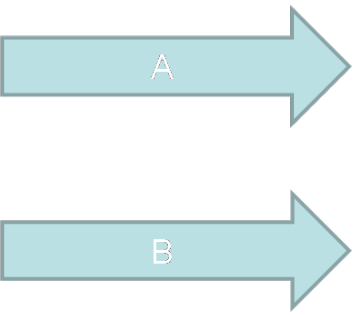
\includegraphics[width=5.5cm]{figs/Verif/parallell.png}
\caption{Parallel data flow}\label{fig:para}
\end{wrapfigure} 

Consider two data flows occurring in parallel. To verify this completely, every scenario must be accounted for. A gets data and not B, B gets data and not A, both A and B or neither. This needs to be accounted for in every clock cycle. In a large design with many operation properties, verification becomes unfeasible even with two parallel data flows.     


Where one draws the conceptual border of a cluster, often falls naturally on the interface between to modules. Sometimes however, it is necessary to do a cluster split where the border consists of arbitrary signals in the middle of a module. Any signal can be determined as an input or output to the completeness plan of a cluster\cite{clust}. When splitting a design into clusters it is important to verify all clusters completely and that any signal that is defined as an input to a cluster is either an input to the design, or an output from another cluster. When defining the signals that represent inputs and outputs between clusters it is recommended to use the same signal names in both clusters. An example of this is using the top level signal in the RTL design that connects cluster A to cluster B. This is to eliminate the possibility that an output from cluster A actually represent a different signal than its respective input to cluster B. By following these guidelines there are no gaps in verification between the clusters. 



\section{Path Predicate Abstraction}
\label{sec:ppa}

This section reviews the principles of PPA and how it is used to abstract the RTL using operation properties. This does not serve as a standalone description of the full theory, for that the reader is referred to \cite{2014-UrdahlStoffel.etal}. To give an intuitive understanding of the abstraction mechanism PPA is discussed with regard to FSM's. Consider an arbitrary RTL design and its accompanying FSM. This FSM has its own input and output alphabet and describes a possibly complex sequence of operations. PPA is used to simplify this sequence of operations by identifying only the important states, a process illustrated with operational graph coloring. \\ 

\begin{figure}[hbt]
\label{fig:ppa}
 \centering
 \begin{subfigure}[b]{0.4\linewidth}
 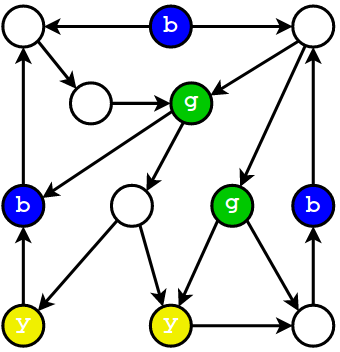
\includegraphics[width=\linewidth]{figs/opcoloring.png}
 \caption{Operationally colored graph}
 \end{subfigure}
 \begin{subfigure}[b]{0.3\linewidth}
 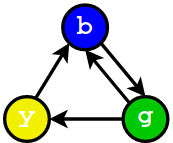
\includegraphics[width=\linewidth]{figs/ppa.png}
 \caption{Resulting PPA}
 \end{subfigure}
\end{figure}

With operational coloring one is able to choose quite freely which states to group together in a conceptual state, and which to leave out as "unimportant" states as long as two rules are followed. 
\begin{enumerate}
 \item All cyclic paths must be broken by at least one colored node, there must be no cyclic path in only uncolored nodes. 
 \item If there is a path between two colored nodes $g\rightarrow y$, there must exist a path to a node of color $y$ from any node of color $g$. 
\end{enumerate} 

Figure \ref{fig:ppa} a) shows the operationally colored FSM of the RTL and b) shows the resulting PPA. It can be easily verified that the color sequence of any path in a) is represented in b). Through abstraction the FSM has been greatly simplified, although some information is lost in the process. It is not possible to extract the original FSM based on the abstraction. An accompanying abstraction of the input and output alphabet of the original must be derived. A communication spanning several nodes in the FSM can now be represented using a single compound in one transition. What before was SDRAM controllers \textit{burst\_read} spanning or 8 more cycles can now be represented as a single operation with $sdram\rightarrow read(compound)$. All transitions between the nodes of the PPA together with the abstract input and output alphabet are formulated in operation properties. This set of properties can now be refined to hold on the original design, and a completeness analysis can be run. As covered in section \ref{subsec:cipc} this verifies the complete I/O behavior of the design, and the set of abstract properties can be said to be a sound abstraction of the RTL.  



\section{Property Driven Development}
\label{sec:pdd}
With the PDD methodology a hardware system is represented at the ESL as a product of time-abstract modules communicating at the transaction level. The individual modules of this ESL are analyzed using a software tool \cite{descam} which generates a complete set of operation properties. The modules are designed at the RTL step by step to make the properties hold on the design. When the complete set of properties hold on the design, the ESL is a sound abstraction of the RTL. For a complete overview of the design flow, case studies and proofs the reader is referred to \cite{pddref}. \par
It is not possible to create sound abstractions of hardware modules using arbitrary SystemC constructs. This is particularly true for time abstract SystemC modules. SystemC-PPA defines a subset of SystemC and dedicated communication channels. A module is described in SystemC as an infinite loop iterating over an FSM, where only 32-bit integers, enums and boolean datatypes are allowed. Collections of these datatypes are allowed in structs, so called compounds. Compounds are used to model communication at the transaction level. Consider a compound containing four data words and addresses. This compound is transferred between two modules in one iteration at the ESL, in contrast to the RTL where it is transferred as a four beat burst. The operation properties are refined such that appropriate address and data words are cycle accurate with respect to the RTL. \par
Communication at the hardware level is divided in two main categories, asynchronous and synchronous. In asynchronous communication transmission is enabled through event signaling, where the receiving end must always be ready to receive such an event. Synchronous communication is enabled through use of a common clock, it is understood through explicit timing that the receiver is ready. There is also the case of unilateral synchronization, where only one communication partner sends such an event. It must then be guaranteed through timing that the other partner is ready. The abstract system model consists of asynchronous PPA's which communicate with each other using events. In SystemC-PPA communication is implemented with channels using port interfaces.


\subsection{Port interfaces}
\label{subsec:ports}       
In SystemC-PPA there is three port interfaces available, two of which model the asynchronous and unilateral synchronization mentioned above. The last provide a means of modeling a volatile memory. 

\begin{enumerate}
 \item \textit{Blocking}: The blocking port models asynchronous communication through a four phase handshake. 
 Two modules communicate using $blocking\rightarrow read()$ and $blocking\rightarrow write()$ where the module calling the function is blocked until the other party signals a synchronization signal. 
 This is implemented in SystemC using $event$ and $wait(event)$. This behavior is represented in the properties by use of $notify$ and $sync$ signals for both parties. 
 Each blocking write or read implies an important state and two properties, one for transfer and one for wait. The wait property proves the system is halted; no state, 
 visible registers or outputs are modified while $sync$ is de-asserted. These event notifiers must be implemented in RTL to satisfy both properties, which carries some overhead. 
 To guarantee that no transmission is lost, each notify/sync must be de-asserted in turn between each transfer. There is also a non-blocking alternative available within the interface, 
 which does not guarantee transmission without explicit timing constraints. As a result the system is not halted and a wait property is not generated when using the non-blocking alternative.
  A non-blocking write will however, in any case hand away control by calling a $wait(arbitrary time)$ after every write. The read on the other only calls such a wait if there is no writer blocked on the port.  
 \item \textit{MasterSlave}: To model the unilateral synchronization a master/slave interface models the case where a master can initiate a transfer at any point without regard. The transfer is guaranteed here because the slave will always be ready to respond to the request. The master will issue a synchronization signal and its SystemC-PPA can be modeled rather freely. On the slave side certain rules apply which $DeSCAM$ will check for. All slave ports must be written in every run and no port can be written twice before all other have been and no slave module can use a blocking interface.
 \item \textit{Shared}: The shared port implements no event synchronization and calls no $wait()$ function. It is meant for modeling unordered input data like sensor values. It can be useful to provide additional information in combination with one of the other interfaces.   
\end{enumerate} 

\section{Related work}
\label{sec:related}
The most notable related work is obviously the case study that is the basis of this thesis. 
The case study is concerned with describing a Wishbone bus architecture at the ESL at two different levels of abstraction. 
Both ESL descriptions have interval properties generated, and each their RTL designed based on these properties. 
The case study shows that a higher level of abstraction leads to substantially faster simulation speed. Furthermore, 
the properties from the abstract design are then refined to hold on the less abstract design showing the flexibility of PDD. 
This feature is what this thesis is based on, representing complex multi level hardware using an abstract ESL. The full case study is available in \cite{pddref}.
(need to elaborate, and bring in the ahb formal verification work too)

\section{The AMBA-AHB}
\label{sec:ahb}

This section is a shorthand guide to the AMBA AHB and its specification to aid in understanding the aspects of the protocol and architecture used in this implementation. For the full AMBA AHB specification refer to \cite{amba}. The AMBA AHB is a pipelined high performance bus architecture supporting multiple masters and slaves. Important aspects of the AMBA AHB are highlighted:

\begin{tabular}{p{3cm} p{10cm}}
Bus master(s) & Can when granted, initiate a transfer, a read or write in the form of a burst or as a single transfer. Multiple master can not transfer concurrently. \\
Bus slave(s) & Responds to the granted master by reading its control signals in one phase, and responding in the next. \\
Arbiter & Chooses which master gets a bus grant by using a chosen arbitration scheme. Relevant schemes are fixed priority and round robin. The arbiter controls the address/control and write data mux \\
Decoder & Decodes the address, selects appropriate slave and controls the response data mux. \\
Default slave & Response given when no valid slave is selected, it is usually integrated in the decoder.\\
Default Master & The arbiter grants a selected default master the bus when idle. \\
\end{tabular}


\begin{figure}[hbt]
    \begin{center}
        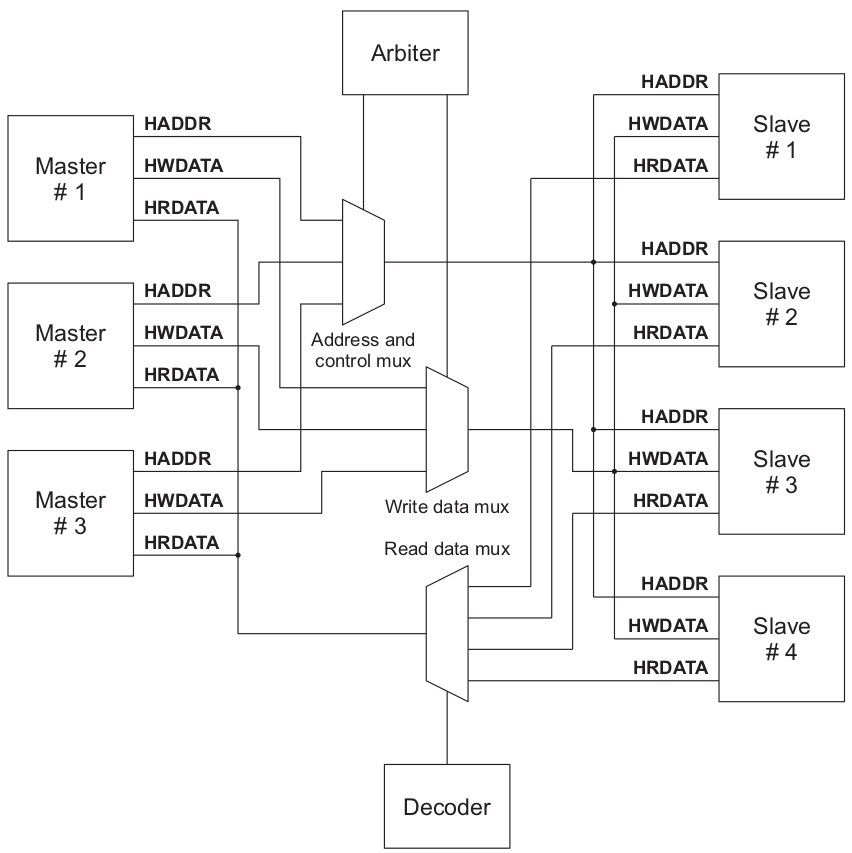
\includegraphics[width=0.8\textwidth]{figs/AHB/AHB_connections.png}
    \end{center}
    \caption{An overview of AHB interconnect, reprinted from \cite{amba}. The mux outputs are referred to as address or data buses.}
    \label{fig:interc}
\end{figure}

\newpage

\begin{figure}[hbt]
 \centering
 \begin{subfigure}[b]{0.4\linewidth}
 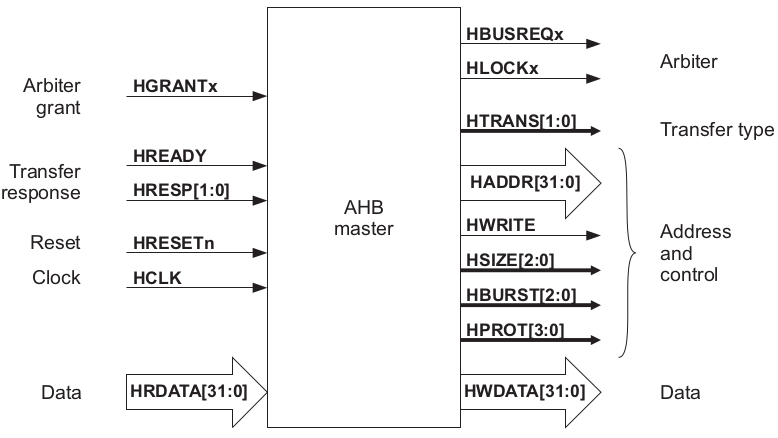
\includegraphics[width=\linewidth]{figs/AHB/master_signals.png}
 \caption{Master signals}
 \end{subfigure}
 \begin{subfigure}[b]{0.4\linewidth}
 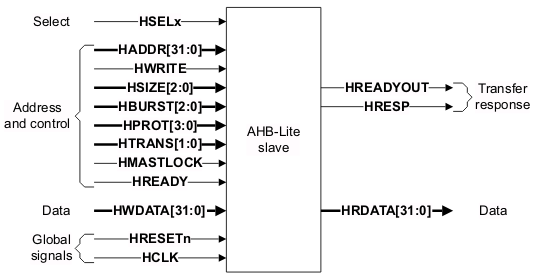
\includegraphics[width=\linewidth]{figs/AHB/slave_lite.png}
 \caption{Slave signals}
 \end{subfigure}
 \caption{Master and slave signals, reprint from left:\cite{amba} right:\cite{amba3}. AHBLite slaves are compatible with AHB systems\cite{ambacomp}. \textbf{HRESP[1:1]} is therefore hardwired to 0.}
 \label{fig:ahbsig}
\end{figure}


As figure \ref{fig:interc} illustrates, the selected address/control and data signals are broadcast to all receivers simultaneously. On the slave side every signal is ignored unless the \textbf{HSELx} signal is set by the decoder. Slave \textbf{x} then reacts to the \textbf{HTRANS[1:0]} and \textbf{HREADY} control signal. Since the master is the initiator it will only react to appropriate signals when expected. \\

\subsection{Transfers}

\subsubsection{Overview of transfer}

\TLSAY{The text below does not provide an overview ... it's very detailed. I would start with a quick overiew of read/write ... I guess you didn't end up working on burst at all? and the show the waveform and explain the hready, hreq and so on with the waveform} 
A master requests the bus by asserting its \textbf{HBUSREQx} signal. The master waits until \textbf{HREADY} and its \textbf{HGRANTx} is set and provides appropriate address and control signals in the next cycle. The transfer is now in the address phase, all set values must be kept valid until \textbf{HREADY} is set. The transfer is now in the data phase. If the transfer is a write, the master must provide valid data and keep it valid until \textbf{HREADY} is set. Otherwise it is a read, and the slave does not need to provide valid data until it sets \textbf{HREADY}. Master samples the data when \textbf{HREADY} is set.
\newpage

\begin{figure}[hbt]
    \begin{center}
        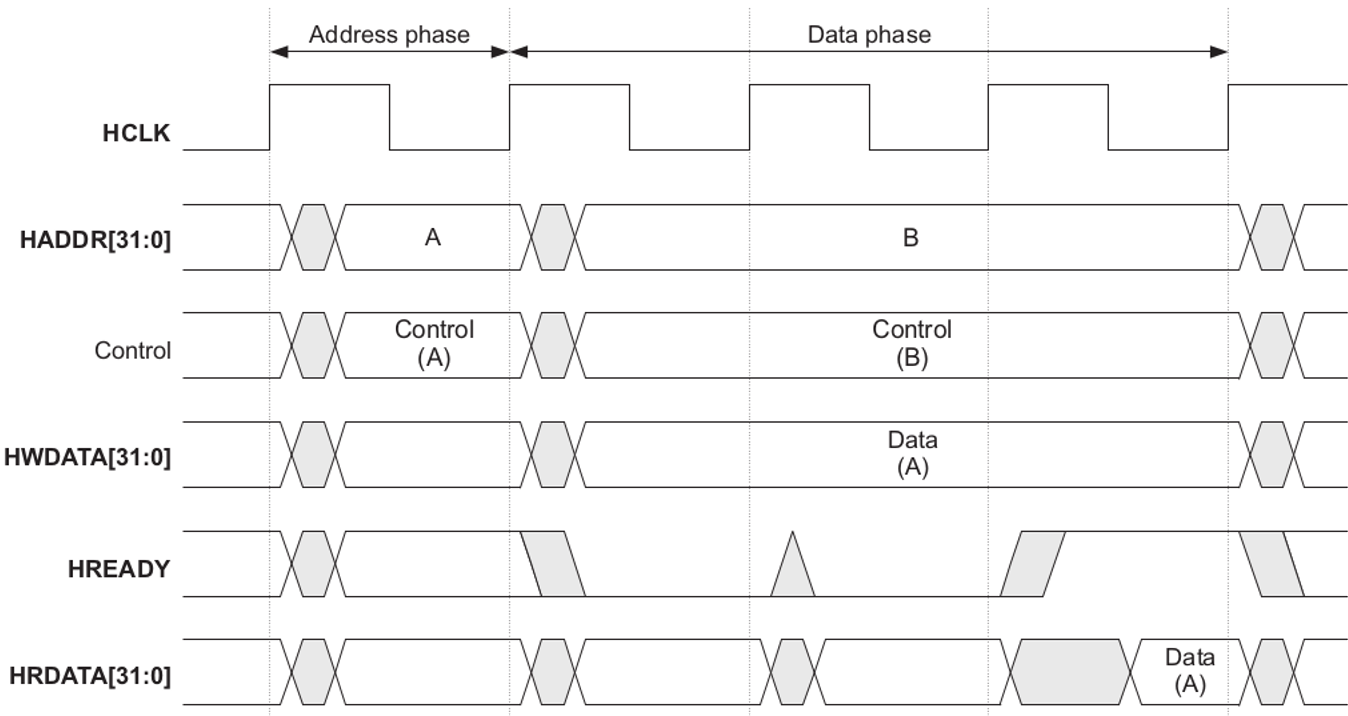
\includegraphics[width=0.8\textwidth]{figs/AHB/transfer.png}
    \end{center}
    \caption{A transfer with wait states, modified reprint from \cite{amba}. In this document the letters represent different masters}
    \label{fig:transfer}
\end{figure}

In figure \ref{fig:transfer} master A initiated a transfer, and the slave extends the data phase to give itself time to handle the request. When the slave is finished it responds using \textbf{HREADYOUT}, \textbf{HRESP} and if it is a read request, \textbf{HRDATA}, see \ref{subsubsec:slvresp}. As seen from the figure, extending the data phase for A has a side effect of extending the address phase for B. B is the address bus owner, but any selected slave knows not to react to its control signals. \textbf{HREADYOUT} is routed back to the slaves input as \textbf{HREADY} through the address mux, and must be set for the slave to sample address and control. For this reason only \textbf{HREADY} is referred to for the remainder of this document. 

\newpage
\subsection{Control signals}
The following signals determine which actions the slaves perfom:
\begin{table}[hbt]
  \label{tab:htrans}
  \begin{tabular}{|p{28mm}|r|p{10cm}|} 
  \hline
  \textbf{HTRANS[1:0]} & \textbf{Type} & \textbf{Description} \\
    \hline
  00 & \textit{idle} & No transfer required, used when a master is granted the bus but does not wish to initiate a transfer. Selected slave must always provide a zero wait state \textit{okay} response and ignore all other signals.\\
    \hline
  01 & \textit{busy} & Used by master to insert idle cycles in the middle of a burst sequence. \\
    \hline
  10 & \textit{nonseq} & Indicates the start of a transfer, address and control is unrelated to the previous transfer. Single transfers are treated as burst of one, the transfer type is therefore nonsequential\\
    \hline
  11 & \textit{seq} & The remaining transfers in a burst are sequential.\\
\hline
  \end{tabular}
\caption{Transfer type}
\end{table}

\textbf{HWRITE} indicates direction of transfer, a write request is performed when set.

\begin{table}[hbt]
  \label{tab:hsize}
  \begin{tabular}{|p{25mm}|r|p{10cm}|} 
  \hline
  \textbf{HSIZE[2:0]} & \textbf{Size} & \textbf{Description} \\
    \hline
  000 & 8 bits & \textit{Byte}\\
    \hline
  001 & 16 bits & \textit{Halfword} \\
    \hline
  010 & 32 bits & \textit{Word}\\
    \hline
  remainder & >32 bits & \textit{not implemented}.\\
\hline
  \end{tabular}
\caption{Data width}
\end{table}

\subsection{Slave responses}
\label{subsec:slvresp}
After a transfer has been started only the active slave has the ability to end it. The active uses \textbf{HREADY} in combination with \textbf{HRESP} to signal the status of the transfer. The slave can either extend and complete the transfer, or provide a two cycle error response. 

\begin{table}[hbt]
  \label{tab:hsize}
  \begin{tabular}{|r|r|p{10cm}|} 
  \hline
  \textbf{HRESP} & \textbf{HREADY} & \textbf{Description} \\
    \hline
  0 & 0 & Wait state\\
    \hline
  0 & 1 & Transfer complete/Okay response \\
    \hline
  1 & 0 & First cycle of error response\\
    \hline
  1 & 1 & Second cycle of error response \\
\hline
  \end{tabular}
\caption{Slave responses}
\end{table}

If the address provided on the address bus is outside the range of any existing slave the default slave response must be provided. If the encoding on \textbf{HTRANS[1:0]} is \textit{idle} or \textit{busy} default slave must provide a zero cycle okay response. Otherwise the default slave must provide the two cycle error response. 






%%%%%%%%%%%%%%%%%%%%%%%%%%%%%%%%%%%%%%%%%%%%%%%%%%%%%%%%%%%%%%%%%%%%%%%%
\chapter{Implementation}
\label{chap:implementation}
\label{ch:impl}
This chapter presents the proposed implementation of the AHB system generator. Sec.~\ref{sec:hardover} provides an overview of the hardware described at the RTL. Sec.~\ref{sec:syslev} discusses how the ESL description is adapted to represent the hardware architecture. The challenges in creating a sound abstraction
of the hardware are elaborated. This is followed by an overview of the simulation models on both levels in Sec.~\ref{sec:sim}. The chapter is ended with Sec.~\ref{sec:results} where results of property checking and simulation times are presented.

\newpage
\section{Hardware overview}
\label{sec:hardover}
\begin{figure}[hbt]
    \begin{center}
        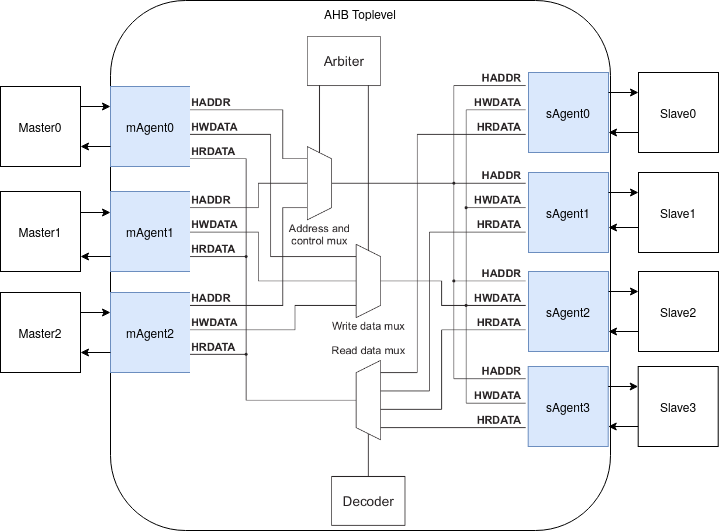
\includegraphics[width=0.8\textwidth]{figs/hw/Hw_toplevel.png}
    \end{center}
    \caption{Hardware top-level with 3 masters and 3 slaves connected}
    \label{fig:hw_toplev}
\end{figure}

For the purpose of this work, it makes little sense trying to implement the AMBA-AHB protocol from scratch starting at the ESL. It would take too much time to design the system and verify that it complies with the protocol. Instead, a trusted existing open source architecture is used. It is trusted in the sense that
it is often referenced when "the how" of protocol implementation is inquired. Furthermore, it has been available for scrutiny online for the last 15 years.  


\subsection{Existing hardware}
\label{sub:exist}
The existing hardware is taken from the \textit{ahb\_system\_generator} found at www.opencores.com \cite{ahbsys}. This architecture is already structured for the
means of generation and is implemented in VHDL, although is doesn't support wide data bus configurations it is the ideal candidate for this work. The master and slave agents was not taken from this source, they were rather redesigned to match SystemC-PPA compliant modules. This architecture supports fixed-priority, round robin and random priority arbitration. There are also modified versions of these arbitrations, where a grant is maintained as long as \textbf{HBUSREQx} is asserted. The chosen arbitration for this work is the modified fixed-priority. The possibility of starvation is a drawback, but it is far less complicated to model at the ESL than for example round robin. Due to limited time, burst, split and retry transfers are not implemented in the agents. The the modified extension to fixed-priority is selected to simplify an implementation of burst transfers. A study of this is presented in chapter \ref{ch:summary}. This hardware is represented in Fig.~\ref{fig:hardover} as the arbiter, decoder and wires connecting the agents. For simplicity it will collectively be referred to as the bus matrix. \par 
For reasons discussed in Sec.~\ref{sec:syslev} a property set was manually described to discover a suitable abstraction of this hardware. In the process it was
discovered that the default slave did not provide a zero cycle OKAY response when it was supposed to. It did however, provide the two cycle ERROR response as 
required by the protocol. This error does not change any functionality of the design, and would never show up in simulation unless a master or agent was sensitive to this. Because it complicated the development of a property set, it was corrected. 

   
\subsection{Master agent}
\begin{wrapfigure}[12]{l}{5cm}
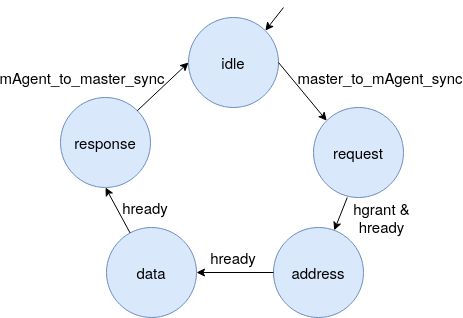
\includegraphics[width=5cm]{figs/hw/mAgent_FSM.png}
\caption{Master agent FSM}\label{fig:rafsm}
\end{wrapfigure}  

The master agent implements the master side of the AHB protocol. It is initialized to the \textit{from\_master} state, where it awaits a payload. The $agent\leftrightarrow master$ interface implements the four phase handshake in both directions. In other words, it is blocked pending a a synchronization signal from the master. The payload represents only a subset of the AHB master interface. The remaining signals are hardwired to default values. \textbf{HTRANS} is an exception, this signal is controlled by the agent throughout the transfer. In an ESL description it is sometimes beneficial to use enums to represent certain encodings and signals. This is to enhance readablility for the designer. These enums have been directly transferred to the RTL description. The entire payload is listed in table \ref{tab:mpayload}, where unchanged signals are marked with a dash.  

\begin{table}[hbt] 
  \label{tab:mpayload}
  \begin{tabular}{|p{25mm}|r|p{10cm}|} 
  \hline
  \textbf{Signal} & \textbf{Type} & \textbf{Content} \\
    \hline
  \textbf{HADDR} & - & - \\
    \hline
  \textbf{HWDATA} & - & - \\
    \hline
  \textbf{HWRITE} & enum & AHB\_READ, AHB\_WRITE \\
    \hline  
\textbf{HSIZE} & enum & MT\_B (byte), MT\_H (halfword), MT\_W (word) \\
    \hline
  \end{tabular}
\caption{Master out payload}
\end{table}

The return payloads consists of only \textbf{HRDATA} and \textbf{HRESP}. A key drawback that is obvious from the FSM is that the agent will return a payload 
to the master regardless of transfer direction. Surely throughput would be higher if the agent bypassed this state in the case of a write. If the transfer
status is not reported back to the master, any error would only be known locally in the agent. It would be possible to assert an error signal that is checked 
before starting a new transfer. However, any predesigned code for a CPU using the AHB protocol i.e linux is likely to expect the error to apply to the current transfer, not the previous. To avoid limiting the bus to systems with manually tailored code, a payload is returned to the master in any case. This comes
at the cost of latency, but as discussed this is a reasonable trade-off. \par
An overview of a transfer is provided with respect to the FSM.
\begin{enumerate}
 \item \textit{from\_master}: Initial/idle state, when a synchronization signal is received, the payload is translated to pure bit and bit vector values and written to the AHB interface.
 \item \textit{Request}: \textbf{HBUSREQx} remains asserted until agent is granted the bus and the bus is ready.
 \item \textit{Address}: \textbf{HTRANS} is encoded with NONSEQ, signalling the start of a transfer. This remains encoded until the bus is ready.
 \item \textit{Data}: When the bus is ready, return payload is read from the AHB interface and written to the master.
 \item \textit{to\_master}: Agent waits for a synchronization signal from the master. The master should already be asserting its synchronization signal, but this is not a requirement.   
\end{enumerate}

The sequence of operations above does not seem to match the sequence in the protocol covered in Sec.~ref{sec:ahb} in the previous chapter. It is however, 
understood that address/control and data can have arbitrary values outside their respective phases, as long as the intended values are present in their 
respective phases. It is therefore also not an issue that they have the intended values outside the respective phases as well. This is provided that \textbf{HTRANS} have the correct encoding at all times.  \WKSAY{Specify that reads and writes are equal if this design desicion remains}
 

\subsection{Slave agent}
\begin{wrapfigure}{l}{5.5cm}
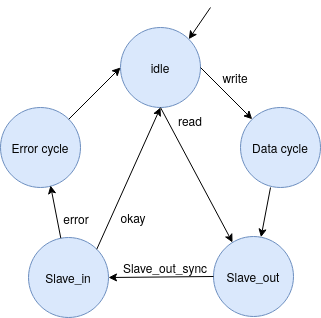
\includegraphics[width=5.5cm]{figs/hw/sAgent_FSM.png}
\caption{Master agent FSM}\label{fig:rsfsm}
\end{wrapfigure}  

The slave agent implements the slave side of the protocol. 

\WKSAY{I think this FSM is misleading, since HREADY=1 is part of the data phase}
As figure \ref{fig:rsfsm} shows the slave agent FSM is more complex than that of the master agent. To make the slave agent comply with the AHB protocol it needs to both obey the rules of the transfer phases and provide the proper response while communicating with its slave. A slave agent is always ready to receive a payload from its master, namely the AHB matrix. \WKSAY{the word phase should not be used for idle in slaves}
Starting from the \textit{idle\_phase} the agent stays idle until it is both selected and the encoding of \textit{nonseq} is detected on its inputs. When true it samples address and control signals from the AHB matrix and proceeds to the \textit{data cycle} where it samples the data. After sampling the data, the payload is written to the slave out port named \textit{sAgent\_to\_slave}. At this point the agent waits for a handshake, which should normally occur instantly but that is not a requirement. After the handshake is received it proceeds to wait for the response data and status from the slave, as with the output there is not a strict requirement on the wait time but it is recommended to keep the wait states under 16 cycles in total. The slave agent deasserts \textbf{HREADY} throughout its entire conceptual data phase, and zeroes \textbf{HRDATA} one clock cycle after asserting \textbf{HREADY}. \\
\newline
\WKSAY{this is highly misleading, it may not be operated by another master, only one can be operated at a time, rather it signals to the bus that it is not ready yet.}
The slave agent may at any given timepoint be operated by another master. This is why the slave deasserts its \textbf{HREADY} throughout its entire conceptual data phase. It is standard for a slave to introduce wait states. As with a DRAM module, there are delays associated with activating a row (insert data). As with DRAM this delay is minimized in sequential address transfers using bursts. In contrast to the diagram in figure \ref{fig:transfer}, the conceptual data phase of the slave agent does not include the assertion of \textbf{HREADY}. 
\WKSAY{what is a misnomer? and dont use the word assertion this way.}
This is a slight misnomer since the data phase does in fact include the assertion as seen from the properties. It is however not included in the FSM to not diffuse the differences between the states. The \textit{idle\_phase} and \textit{error cycle} only differentiate in the value of \textbf{HRESP}. Although the assertion of \textbf{HREADY} technically is a part of the data phase, it is however beneficial to highlight that these are separate states, as they are represented as such in the RTL description. The zeroing of \textbf{HRDATA} is a design choice to increase abstraction. \WKSAY{Why does this increase abstraction, this hangs a bit loose}
\newpage

\section{System level representation}
\label{sec:syslev}
\begin{figure}[hbt]
    \begin{center}
        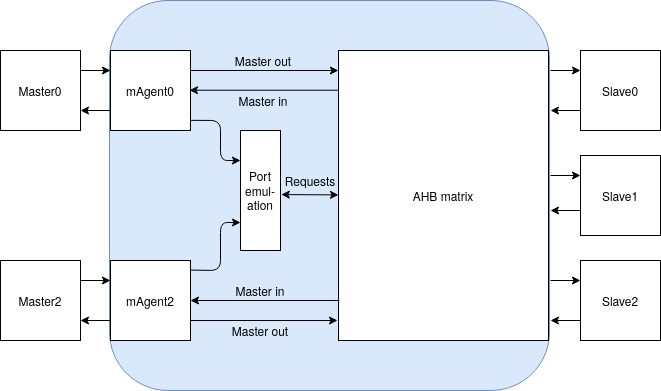
\includegraphics[width=0.8\textwidth]{figs/ESL/Syslev.png}
    \end{center}
    \caption{ESL toplevel with 2 masters and 3 slaves connected}
    \label{fig:esl_toplev}
\end{figure}

When representing the AHB system at the ESL, abstraction is a priority. Ideally there would be a single SystemC-PPA describing the entire system. It is on 
the other hand not possible to represent this multi-master design without separating the master agents into their own SystemC-PPA. The reason for this is 
parallelism, and a single threads lack of capability to represent it. Regardless of which conceptual state the system is in, any idle master can receive 
a message and proceed to request. This operation requires the modification of the output \textit{mAgent\_to\_master(x)\_notify} in addition to knowledge of this
request at the next conceptual system state. This is not practical to represent at the ESL, if it is even possible. Considering that the ESL needs to represent an existing RTL description, it is beneficial to manually write the properties bottom-up to get an idea of how the system level description must be formed.

\subsection{Manual property set}
During the development of the initial property it became clear that to determine the state of the bus, knowledge of past behaviour is required. It is not possible to determine only by observing the internal registers of the design. It is easy to determine which master owns the address and
data bus. However, this provides little information when the operating master is the default master. Even when observing the encoding on \textbf{HTRANS}, it is impossible to determine if the default master is active or idle in the data phase. One alternative is to look at past values of \textbf{HTRANS} to determine if the default master recently was in the address phase. Another much simpler alternative is to exploit that master agents are verified in separate clusters. The
state of the master agents are determined as outputs to their clusters and as inputs to the main cluster. The state of the bus is now possible to determine at any time by observing the states of the master agents. \par
The next steps in developing a complete property set include discovering visible registers and determining outputs to the design. Most of the important signals
in this design are updated on a clock edge, which is straightforward to represent at the ESL. One of the signals of the master interface, \textbf{HGRANTx} is 
not updated on a clock edge. This is problematic because it is not feasible to determine a fixed value for this signal in the next time point. \textbf{HGRANTx} 
must be updated with the output of a function. For the same reason, the signals on the address bus can not be represented directly. The visible registers 
representing the address bus are rather the inputs from the master agent in the state \textit{Address}, and if none apply a default value is selected. 

\subsection{Forming the ESL}
 




\WKSAY{Describe in detail the problem with multi-master designs, then describe in detail key things that must be represented in the ESL, like hready and hgrant in terms of the phases. They must be determined}
Describing the AHB system with SystemC-PPA in a single cluster is no longer feasible when more than one master is connected to the bus matrix. The master agents must be contained within their own clusters, or PPAs so that it does not need to be accounted for every possible combination. Since only one slave may be operated at a time, including them in the bus matrix PPA reduces the overhead. The interface between the master agent and the bus matrix have signals with mostly identical values for all masters, the exception is \textbf{HGRANTx}. This signal is purely combinational in the implementation, meaning that it changes its value within the same clock cycle as its initiator. Using any combination of existing ports there was not found any manner to represent this interface for multiple masters. The decision was made to create the properties bottom-up, to determine if the interface could be represented using existing ports and if not, where the gap is. Gap free verification was used for this purpose, with the style of generated properties in mind. 

\subsection{Bottom-up abstraction}
\WKSAY{bottom up properties}
The first challenge of carrying out the GFV process is determining the CSM of the AHB. It has to be represented in such a way that it is feasible to describe at the ESL. Looking at other formal verification efforts made on the AHB \cite{ahbformal}, it can be seen that the real FSM of an AHB is incredibly complex. 
\WKSAY{it is incredibly complex because of burst} Furthermore, it is described how the state of the bus is dependent not just on state and inputs but on previous states as well. It is necessary to know the state of the bus, namely if there is a transfer being carried out or not. It is not as simple as paying attention to bus ownership since there is no way of knowing if there is a transfer in progress when the default master owns the data bus, without looking at past values on \textbf{HTRANS[1:0]} \WKSAY{long and useless sentence, this whole thing should be rewritten}. One would furthermore need to constrain the design to establish how far into the past to look. One could go with the suggested maximum delay of slaves for 16 clock cycles. A much simpler solution is to define the master agents states as outputs to their clusters, and define this as inputs to the main cluster. By only concerning with which masters are requesting and where the data goes, the CSM can be made quite simple. If one was concerned with which master owned the address and which master owned the data bus at all times it would lead to state explosion, making an ESL description unfeasible even for a low number of masters.     

\begin{figure}[ht!]
	\centering
	\begin{minipage}[t]{0.49\textwidth}
		\centering
		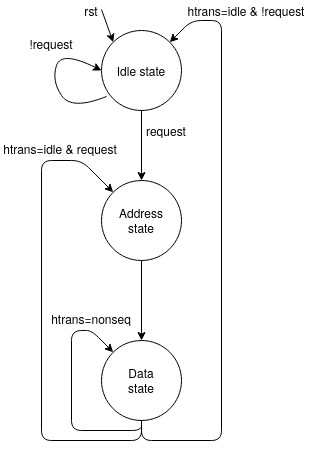
\includegraphics[scale=0.5]{figs/ESL/Bus_fsm_new.png}
		\captionof{figure}{Abstract CSM}
		\label{fig:OC}
	\end{minipage}
	\begin{minipage}[t]{0.49\textwidth}
		\centering
		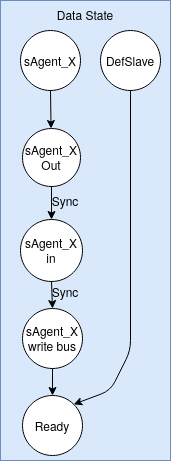
\includegraphics[scale=0.5]{figs/ESL/Data_state.png}
		\captionof{figure}{Detailed data state CSM}
		\label{fig:eslfsm}
	\end{minipage}
\end{figure}


By using a fixed priority arbitration scheme it is simple to determine which master is granted the bus. 
\WKSAY{This is nonsense, it needs to be restructured, be more descriptive, separate ESL states from property states}
By dividing the transfer into three main states with the data state divided into five further, there is no need to impose any constraints on wait states. The bus is ready (\textbf{HREADY} is set) at the end of each state and any request is ignored unless the bus is ready. The states can be defined as follows:
\begin{itemize}
\item Idle state: No transfer in progress.
\item Address state: One master is in the address phase of the transfer, no masters are in the data phase. There is no trigger for the next state as the bus/slaves will always be ready here. 
\item Data state: One master is in the data phase of the transfer. This state is broken down into five substates per slave, with default slave as exception.  
\end{itemize}


\WKSAY{This does not describe the bottom up properties, it describes the actual properties. you need to separate that}
It is worth noting that in the idle and address state the bus/slaves are always ready. The payload is transferred between the states using visible register which are named \textit{AS\_regs} for the address state and \textit{DS\_regs} for the data state. The Data state is divided into several important states to describe the transaction between the slave and its agent while simultaneously describing all necessary outputs. The default slave has only two states and they are self explanatory because of the two cycle error response. The remaining slave agents are explained by the following:
\begin{itemize}
 \item First state: There is one clock cycle delay required to allow the slave agent time to sample the possible data provided in the data phase.
 \item Second state: Slave agent writes payload to slave using blocking write. 
 \item Third state: Slave agent reads back from slave using blocking read.
 \item Fourth state: Slave writes payload back to bus. This requires two cycles due to the possibility of error, error cycle was removed from master agent due to inconsistencies in simulation. For this reason information on error is only contained within the visible registers handling response.   
 \item Fifth state: The bus is ready, payload is sampled, requests are handled and next state is determined based on the value of \textbf{HTRANS[1:0]}, which has been added to \textit{AS\_regs} alongside the payload. 
\end{itemize}

It is easy to see that the differentiation between read and write within the AHB matrix would lead to the double amount of data states \WKSAY{consider the trade-off, is it worth it?}, with the gain being one clock cycle saved in the case of a read \WKSAY{confusing and also probably wrong}. The entire design is represented by this CSM using only properties with length $t=1$ \WKSAY{t is the arbitrary timepoint, t=everything, use t\_end or something}so determining the output is straightforward with the exception of \textbf{HGRANTx}. As this is an output that is not stored in a register its value updates in the same clock cycle as its \WKSAY{is instrigator the word?} instigator. This is not a problem to model in the properties themselves, but this representation does not allow for any sound abstraction between the RTL and ESL \WKSAY{rather say it is not possible to represent by assigning value to a variable}. Determining the value of \textbf{HGRANT} in the next clock cycle is not feasible in this implementation. One would have to account for every \textbf{HBUSREQx} as an assumption at $t+1$ in every property. An alternative could be to enable this output through a register but this would lead to unpredictable behavior. This output is simply determined as the output of a function \textit{mx\_grant} and is at the ESL represented using an enum. \\
\newline
The design choice to zero \textbf{HRDATA} and modify the default slave response entails that \textbf{HRDATA} and \textbf{HRESP} will be zero unless it is in the fourth or fifth conceptual data state \WKSAY{this sentence is garbage}. After adding all determination requirements and proving completeness the properties show that the interface between the master agents and AHB matrix cannot be represented using a single existing SystemC-PPA port. Referring back to section \ref{subsec:ports} there is a choice between three ports. For clarity the implications of using each port is commented.
\begin{itemize}
 \item \textit{Shared}: Explicit synchronization is needed to ensure that the value of \textbf{HREADY} and \textbf{HGRANTx} is neither overwritten nor obsolete. A solution was experimented with to highlight the increased abstraction. It was not successful without introducing illegal statements with respect to SystemC-PPA, even when disregarding the combinational response of \textbf{HGRANTx} \WKSAY{rather refer to abstraction, and grant}.   
 \item \textit{MasterSlave}: With MasterSlave some implicit synchronization is enabled. However, in this system one would be left with one of two choices. The bus matrix is the slave, or the master agents are the slaves. In either case the values of \textbf{HGRANTX} and \textbf{HREADY} would need to be representing correct values in every cycle. One side must always be ready for communication, so neither alternative is worth considering \WKSAY{rather refer to abstraction, and grant}.  
 \item \textit{Blocking}: The blocking port can be used to represent all signals functionally, but with blocking ports alone there are some issues. On the master agent side \textbf{HBUSREQx}, \textbf{HGRANTx} and \textbf{HREADY} can be represented both functionally and in the properties by the notify and wait used for synchronization. On the bus matrix side the functionality could be represented, but not the properties due to the states implied by each port. They all require their own state, and in turn a separate clock cycle to assert and deassert these signals.
\end{itemize}

The remaining option is to emulate a single compound port using a combination of shared and blocking ports.

\subsubsection{Combinatory port emulation}
When examining the FSM in figure \ref{fig:rafsm} it is seen that the traversal of the master agent state machine is always blocked by an input signal. The \textit{Request-}, \textit{Address-} and \textit{Data\_phase} are blocked by the AHB matrix's response signals \textbf{HREADY} and \textbf{HGRANTx}. Although the value of \textbf{HGRANTx} is impossible to determine effectively in the next clock cycle, its functionality with respect to the state machine can still be properly represented using a blocking port. The handshake from the master agents side represent the request, whereas the handshake from the AHB matrix side represent \textbf{HGRANTx} and \textbf{HREADY}. 
\WKSAY{This sentence is not too clear, requests need to handled in each phase}
Due to the pipeline nature of the bus, a request can occur at any main state of the bus as seen from figure \ref{fig:OC}. This creates the requirement of a separate output representing \textbf{HREADY} alone, to allow for state machine traversal after bus has been granted. Only one port read can be represented in each clock cycle for blocking ports. Due to each master agent requiring their own port for each of the cases, it is necessary to contain these ports in a separate module, and treat it as a new type of port interface.
This port determines internally which master agent gets granted/unblocked with a simple fixed priority arbitration scheme. The final issue is having the port correctly represent updated requests. For this reason the port waits for a synchronization signal (handshake) from the AHB matrix. When this handshake is received the port peeks on all its request inputs and forwards this information to the AHB matrix through a \textit{Shared} interface, while simultaneously unblocking the highest priority requesting agent and every \textbf{HREADY} port waiting for a synchronization signal. Special care has been taken to ensure that this happens in an atomic and synchronized manner.   
\begin{wrapfigure}{l}{5.5cm}
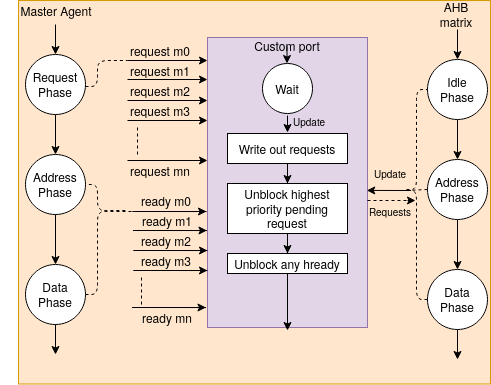
\includegraphics[width=5.5cm]{figs/ESL/port_diagram.png}
\caption{Illustration of port connection}\label{fig:cport}
\end{wrapfigure}

The port in figure \ref{fig:cport} is illustrated using the actual port directions in the ESL description, rather than the direction they symbolize. The inputs representing \textbf{HREADY} must be atomically unblocked which only happens when there is a pending handshake. To check for this the \textit{peek} function must be called, which is only available for reader ports. On the AHB matrix side the synchronization call to update the requests must always hand over control to the port by use of a wait function, which is only unconditionally called by use of a write port. When control is handed back to the AHB matrix the updated requests can be fetched from a shared port. 
\WKSAY{Consider if the port can include the payloads back and forth, although this is harder for burst due to the shared ports}

\subsubsection{Master agent}
\begin{wrapfigure}{l}{5.5cm}
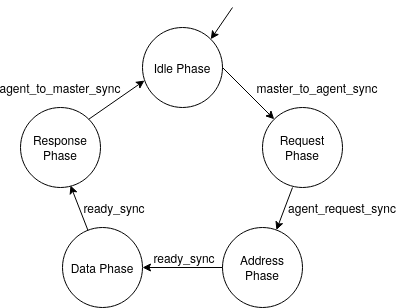
\includegraphics[width=5.5cm]{figs/ESL/mAgent_ESL.png}
\caption{master agent FSM}\label{fig:eafsm}
\end{wrapfigure}
The master agent is modeled at the ESL in a relatively simple manner using blocking ports to determine important states. All states from figure \ref{fig:rafsm} are deemed important states. They are all needed to communicate with the individual states of the bus matrix, or their masters. Transitions between the states are dependent on the synchronization signals alone, and all remaining interface signals are passed through shared ports. The generated properties are refined with minimal effort and proven to be a sound abstraction of the master agent RTL.  \\
\newline  

\subsubsection{Bus matrix}
The bus matrix has three main states as seen from figure \ref{fig:OC}. There is only one single communication with the emulated port in each of the three states. 
\begin{lstlisting}
   update_requests->try_write(true, sync, "idle_state");
   requests_in->get(reqs);
\end{lstlisting}

The sequence allows the emulated port to fetch most recent request from the master agents and update the shared port while the bus matrix is waiting. 
Even though requests are arbitrated within the port to ensure correct functionality, arbitration is again represented with an if then else cluster to represent this behavior in the properties. 
If there are no requests this state will loop, which is preferable to using a blocking write. The wait property associated with the blocking write is impossible to prove due to the possible immediate change of \textbf{HGRANTx}. \par
The payload of the highest priority request is stored in the compound \textit{AS\_regs}, and the bus proceeds to the address phase. (TODO: change bus state to phase, and master phase to state, more clear) 
The compound \textit{AS\_regs} represent the signals broadcast to the bus by the granted master, and is represented in the properties as visible registers. \par
In the address phase the values of \textit{AS\_regs} are stored in \textit{DS\_regs} and the operations in the previous phase are repeated, but without the possibility of a loop.
As seen from Fig.~\ref{fig:OC} the transition to the data phase is unconditional, as all slaves are required to be ready. The data phase is split into a series of substates as seen in Fig.~\ref{eslfsm}.
Since the master agent interface is represented using mostly shared ports, outputs must be written every clock cycle to successfully prove completeness. The properties generated for the shared outputs
are only defined at the right hook. In this case it is not sufficient for properties spanning more than one clock cycle. \par
The request sequence is again carried out, with the difference that it can transition to either of the three states. 
 

\subsection{Refining properties}
\label{sub:refine}
(gotta mention master agent state somewhere)
This section is an overview of the refinement of the properties, and the completeness proof. The interface to the master agents will be covered for both sides in parallel.
The signals \textbf{HREADY}, \textbf{HGRANTx} and \textbf{HBUSREQx} are represented with multiple macros in the property suite, which require explanation. 
\textit{update\_requests} represent all three signals functionally at the ESL, but the generated macros are not sufficient to prove completeness.
The macros needed to fullfil the requirements are listed in Fig.~\ref{fig_reqmac}, where superflous signals are omitted. 

\begin{figure}[hbt]
	\centering
	\begin{minipage}[t]{0.49\textwidth}
		\centering
                 \begin{enumerate}
                   \item \textit{reqs\_sig\_m(x)\_request}
                   \item \textit{update\_requests\_notify}
                   \item \textit{update\_requests\_sync}
                   \item \textit{bus\_to\_mAgent(x)\_sig\_hgrant}
                   \item \textit{m(x)\_grant}
                 \end{enumerate}
              
	\end{minipage}
	\begin{minipage}[t]{0.49\textwidth}
		\centering
		 \begin{enumerate}
                   \item \textit{mAgent\_request\_notify}
                   \item \textit{mAgent\_request\_sync}
                   \item \textit{bus\_ready\_sync}
                   \item \textit{bus\_to\_mAgent\_sig\_hgrant}
                 \end{enumerate}
              
	\end{minipage}
\caption{List of macros for request handling, with bus matrix on the left and master agent on the right}
\label{fig:reqmac}
\end{figure}

\newpage
Brief descriptions of the signals are given in table \ref{tab:reqmac}.

\begin{table}[hbt] 
  \label{tab:reqmac}
  \begin{tabular}{r p{10cm}} 
  \hline
  Matrix & Description \\
    \hline
  \textit{1.} & represents \textbf{HBUSREQx}, macro is determined as input in the completeness description \\
    \hline
  \textit{2.} & represents \textbf{HREADY} "or" (\textbf{HREADY} "and" \textbf{HGRANTx}). Macro is determined as output in the completeness description. This is sufficient to determine \textbf{HREADY}, but not \textbf{HGRANTx} \\
    \hline
  \textit{3.} & represents the "or" of all \textbf{HBUSREQx}, not part of completeness description, but added to table to provide consistency with 1. in agent. \\ 
    \hline
  \textit{4.} & represents \textbf{HGRANTx}, this signal is redefined as boolean and defined as output in the completeness description. \\
    \hline
  \textit{5.} & A function that calculates the current value of \textbf{HGRANTx} based on determined inputs and outputs \\
    \hline
  Agent & Description \\
    \hline
  \textit{1.} & represent \textbf{HBUSREQx}, defined as output in completeness description. \\
    \hline
  \textit{2.} & represents \textbf{HGRANT} "and" \textbf{HREADY}. Is not part of completeness description, but added to table to provide consistency with 2. in bus matrix. \\
    \hline
  \textit{3.} & represents \textbf{HREADY}, defined as input in completeness description \\
    \hline
  \textit{4.} & represent \textbf{HGRANTx}, redefined as boolean. Defined as input in completeness description. \\
    \hline  \end{tabular}
\caption{Description of macros for request handling}
\end{table}

The signals added to provide consistency are not strictly needed to pass any of hte completeness tests. It is rather a security measure to comply with the guidelines for working with clusters mentioned in 
Sec.~\ref{sub:clust}. Although the interface signals are not represented indentically on both sides, as long as the behavior is guaranteed within the emulated port it will not leave a gap in verification.

\subsubsection{Visible registers}
(only matrix)
The macros representing visible registers in the property suite are all variables in the ESL description which store values between the states. In this implementation none of the visible registers directly represent actual registers in the design. They represent input/outputs from/to masters and slaves, based on selection criteria. The selection criteria are generally the states of the master agents, or the conceptual state of the bus. 
\begin{itemize}
 \item \textit{AS\_regs}: Represents the subset of master agent outputs included in the payload, including \textbf{HTRANS} for the agent in its address state. If none it has default values.
 \item \textit{DS\_regs}: Either represents the subset of master agent outputs included in the payload for the agent in its data state. Or represents the output of the slave that has its out notify set. The address offset is effectively accounted for this way. If none apply it has default values
 \item \textit{resp}: Represents the response payload of the slave that has both its in notify and sync set the last 2 cycles. Otherwise it has default values.
 \item \textit{phase/nextphase}: Represents the main CSM of the bus matrix. Selected based on which state macro is true.
\end{itemize} 

(this all sucks but i definitely need to add that the completeness was initially done using only original I/O)


\section{Simulation}
\label{sec:sim}
Simulation models carrying out the same operations are designed for both abstraction layers. One of the main benefits of modeling hardware at the ESL is simulation speed, so a time comparison is carried out between the two layers. Designing two corresponding simulation models also offer some verification. 
The aim of PDD is to do away with RTL simulation all together, but when the ESL description is modeled after an existing hardware architecture it makes sense
to ensure that the two simulation models behave equivalent. \par
Master and slave dummies are connected to the bus matrix. The dummies perform simple operations to maintain a good overview of the operations. 
The masterdummy alternates between single read and writes. It increments the address by 10 every transaction, and the data by 1 every write. 
The simulation lasts for the duration of $10^6$ transfers, during which the address wraps around to 0 if it reaches the end of the slave address range. \par
Assertions are used to control that data is transmitted between the intended dummies. The slave dummy has no information about which master it is operated by. 
All masters can act independently from each other, and due to the arbitration it is not so simple to monitor from a top level perspective. It is an error prone
process and it is avoided. Instead, slaves also store their response in a map. The master asserts that the slave it intended to operate is the one that responds. VHDL offer no such high level functions for monitoring, so one part of the protocol is exploited. To recapitulate; A slave ignores \textbf{HWDATA} for reads, and masters ignore \textbf{HRDATA} for writes. This does not forbid any value being present on the signals for testing purposes. The master asserts
that the same data it writes to the slave is the same that returns. \par
Accessing the default slave does not increment the transfer count, so choosing a non continuous address range will affect the simulation time.  

\subsection{Starvation}
The downside of fixed priority arbitration is that there is no guarantee that every master is granted access to the bus. It is important that this feature is
accurately reflected in the ESL model. There are configurations of masters and slaves attempting to carry out a set of certain tasks where one or more master are never granted access to the bus. This type of configuration is useless and it defeats every purpose of fully verfifying at the ESL if this is not accurately reflected there. \par
The easiest example of starvation to observe is when all master dummies poll the bus. At the RTL, if the masters are requesting within the slave range a fourth master starves Whereas if they request outside the range it is the fifth master that starves. At the ESL on the other hand, it is the fourth master that starves
in either case. It is observed that this is due to an exactly three clock cycle delay, not present in the ESL simulation. This is impossible to model using "zero time" increments, but can be modeled by waiting exactly three times the minimum time increment after response from a master agent is received. This is provided that the minimum is above zero. \par
Will a full system still be represented correctly? maybe the fact that you dont know, if you have a system with many masters use RR.



\section{Generator}
\label{sec:generator}
The AHB system can be generated using a program implemented in C++, where the number of masters and slaves are required as input arguments. Allowed number of
masters and slaves are between 1 and 15. An ESL and RTL description, including testbenches are generated followed by a set of operation properties and completeness descriptions. Two short scripts are included which enable the property and completeness check to be carried out with just one command from the
command line. 

\subsubsection{Automatic property refinement}
The SystemC-PPA descriptions of the bus matrix and master agent are analyzed with the tool DeSCAM. The tool parses the SystemC-PPA and generates an abstract
model and properties. A plugin to the tool has been developed, which is tailored to the SystemC-PPA of the bus matrix and master agent. The plugin iterates 
over the abstract property set, and writes the property set to a file. The plugin inserts the appropriate signal names and logic in the macros as it is written.
 

\section{Experimental results}
\label{sec:results}





%%%%%%%%%%%%%%%%%%%%%%%%%%%%%%%%%%%%%%%%%%%%%%%%%%%%%%%%%%%%%%%%%%%%%%%%
% \chapter{Performance analysis}
% \label{chap:performance}
% \input{performance_analysis.tex}

%%%%%%%%%%%%%%%%%%%%%%%%%%%%%%%%%%%%%%%%%%%%%%%%%%%%%%%%%%%%%%%%%%%%%%%%
\chapter{Summary and outlook}
\label{chap:summary}
In Sec.\ref{sec:sum} of this chapter, the work presented in chapter \ref{ch:impl} and \ref{ch:design} is summarized. Some thoughts on the implementation and areas of further research are given in Sec.~\ref{sec:outl}. The conclusion of this thesis is given in Sec.~\ref{sec:concl}.

\section{Summary}
\label{sec:sum}
This thesis proposes a generator which generates corresponding models of an AMBA-AHB bus architecture at the Electronic System Level and Register Transfer Level for a selected number of masters and slaves. The ESL description is comprised of two SystemC-PPA modules, one of the master agent and one of the bus matrix, which are used to generate complete sets of operation properties which are automatically refined to prove that the SystemC-PPA modules are sound abstractions of their RTL counterparts. The ESL model and agents implement a subset of the AHB protocol, namely single transfers with split and retry responses disabled. \par
An emulated port handles the parallel nature of the interaction with the master agent interfaces. This port is implemented using existing SystemC-PPA ports. This emulated port ensures correct functional simulation and a set of properties which can be proven on the bus matrix. A generated property set cannot be proven for the emulated port interface itself which leaves a gap in verification. A simple arbitration scheme, namely fixed-priority arbitration is chosen such that soundness with respect to the system level is achieved through careful design of the port. \par
The choice of fixed-priority arbitration leaves lower priority masters vulnerable to starvation. The thesis addresses this problem and provides a graphical comparison of starvation between the two models. \par
Simulation models were generated to compare the two models for a range of configurations. The experimental results show the simulation time is reduced by orders of magnitude in the ESL model compared to the RTL model. \par 
Burst transfers are only shown as a proof of concept due to time constraints, since the level of complexity for implementing this is high. The proof of concept is a four-beat incremental burst implemented on a system comprised of a single master and slave. This demonstration shows that burst transfers can be implemented with some limitations. Proving completeness on a design with burst transfers is feasible. \par
 

\section{Outlook}
\label{sec:outl}
Much has been achieved in this work with regards to generating an AMBA-AHB at the ESL and RTL. The individual modules which represent the master agent and bus matrix at the ESL are formally proven to be sound abstractions of their RTL counterparts. Due to the required emulated port interface it still remains to formally prove that the ESL model is a sound abstraction of the RTL model with respect to the system as a whole. Furthermore, a method to model or monitor the starvation should be implemented.    

\subsection{Suggested improvements}
\label{sec:impr}
\subsubsection{Signal name map}
The plugin which refines the properties rely on matching signal names between the models and conditional statements to refine the signal macros. A suggested improvement is to rely on a map which returns the appropriate refinement based on the abstract signal name. The generator would rely on the same map to name the signals such that the model can be configured with more flexibility


\subsection{Further research}
\subsubsection{Formally proven $agent\leftrightarrow bus$ interface}
More research is required on how to formally prove the interface between the master agent and bus matrix. This may be a complex but general solution which implements different arbitration schemes within a SystemC-PPA port interface that can be used in any arbitrated bus architecture. It can be envisioned as a port reader which can have many writers connected. The reader issues two notify events, one is unconditional and signals bus is ready, the other is conditional and signals grant. How arbitration is tackled remains to be determined. It will likely still need to be represented in both the port and in the module implementing the port reader. Perhaps a tool can verify that the arbitration scheme in the model is equivalent to the arbitration scheme in the port. This way, more complex arbitration schemes like round robin can be safely implemented.  

\subsubsection{Monitor starvation}
It was shown that starvation is neither adequately represented or over approximated in the simulation model. A monitor could be implemented, but it requires more research into how this is done. Theoretically, it can monitor the amount of simulation time, or number of context switches within each master between each transfer. If it is not guaranteed that the master which is granted in the ESL model will be granted in the RTL model, the simulation issues a warning or halts the simulation. Some restrictions must apply, such that any context switch or simulation which is counted by the monitor equates to at least one clock cycle in the RTL. Furthermore, some restrictions must be applied to how many wait cycles a slave can insert.    


\section{Conclusion}
\label{sec:concl}
Two goals were set in chapter \ref{ch:intro} of this thesis. This work shows the requirements for generating an abstract representation of the AMBA-AHB with SystemC-PPA. It is possible to generate the system at the ESL and RTL and automatically refine the properties such that they hold on the design. The final system implements single read and write transactions with split and retry response types disabled. Burst transactions are shown to be possible through a proof of concept. Simulations of both models show that all configurations of the ESL model are at least ten times faster than any configuration of the RTL model. More work needs to be carried out to implement the burst transactions in the generator. More research remains to formally prove soundness of the interface between the master agent and bus matrix. To ensure soundness of configurations with more than three masters, a monitor must be implemented.  






     





% %%%%%%%%%%%%%%%%%%%%%%%%%%%%%%%%%%%%%%%%%%%%%%%%%%%%%%%%%%%%%%%%%%%%%%%%
%if you have an appendix put it here
%\begin{appendix}
%   \chapter{Xxx}\label{app:xxx}
%   \input{app_Xxx.tex}
%\end{appendix}
% %%%%%%%%%%%%%%%%%%%%%%%%%%%%%%%%%%%%%%%%%%%%%%%%%%%%%%%%%%%%%%%%%%%%%%%%

\backmatter
\listoftables
\listoffigures 
%\lstlistoflistings

%%%%%%%%%%%%%%%%%%%%%%%%%%%%%%%%%%%%%%%%%%%%%%%%%%%%%%%%%%%%%%%%%%%%%%%%
\bibliographystyle{unsrtnat}
\bibliography{literature}

\end{document}

